\documentclass[dissertation,copyright]{uathesis}
\usepackage[]{graphicx}\usepackage[]{color}
%% maxwidth is the original width if it is less than linewidth
%% otherwise use linewidth (to make sure the graphics do not exceed the margin)
\makeatletter
\def\maxwidth{ %
  \ifdim\Gin@nat@width>\linewidth
    \linewidth
  \else
    \Gin@nat@width
  \fi
}
\makeatother

\definecolor{fgcolor}{rgb}{0.345, 0.345, 0.345}
\newcommand{\hlnum}[1]{\textcolor[rgb]{0.686,0.059,0.569}{#1}}%
\newcommand{\hlstr}[1]{\textcolor[rgb]{0.192,0.494,0.8}{#1}}%
\newcommand{\hlcom}[1]{\textcolor[rgb]{0.678,0.584,0.686}{\textit{#1}}}%
\newcommand{\hlopt}[1]{\textcolor[rgb]{0,0,0}{#1}}%
\newcommand{\hlstd}[1]{\textcolor[rgb]{0.345,0.345,0.345}{#1}}%
\newcommand{\hlkwa}[1]{\textcolor[rgb]{0.161,0.373,0.58}{\textbf{#1}}}%
\newcommand{\hlkwb}[1]{\textcolor[rgb]{0.69,0.353,0.396}{#1}}%
\newcommand{\hlkwc}[1]{\textcolor[rgb]{0.333,0.667,0.333}{#1}}%
\newcommand{\hlkwd}[1]{\textcolor[rgb]{0.737,0.353,0.396}{\textbf{#1}}}%
\let\hlipl\hlkwb

\usepackage{framed}
\makeatletter
\newenvironment{kframe}{%
 \def\at@end@of@kframe{}%
 \ifinner\ifhmode%
  \def\at@end@of@kframe{\end{minipage}}%
  \begin{minipage}{\columnwidth}%
 \fi\fi%
 \def\FrameCommand##1{\hskip\@totalleftmargin \hskip-\fboxsep
 \colorbox{shadecolor}{##1}\hskip-\fboxsep
     % There is no \\@totalrightmargin, so:
     \hskip-\linewidth \hskip-\@totalleftmargin \hskip\columnwidth}%
 \MakeFramed {\advance\hsize-\width
   \@totalleftmargin\z@ \linewidth\hsize
   \@setminipage}}%
 {\par\unskip\endMakeFramed%
 \at@end@of@kframe}
\makeatother

\definecolor{shadecolor}{rgb}{.97, .97, .97}
\definecolor{messagecolor}{rgb}{0, 0, 0}
\definecolor{warningcolor}{rgb}{1, 0, 1}
\definecolor{errorcolor}{rgb}{1, 0, 0}
\newenvironment{knitrout}{}{} % an empty environment to be redefined in TeX

\usepackage{alltt}
\newcommand{\SweaveOpts}[1]{}  % do not interfere with LaTeX
\newcommand{\SweaveInput}[1]{} % because they are not real TeX commands
\newcommand{\Sexpr}[1]{}       % will only be parsed by R


%\documentclass[dissertation,CC-BY]{uathesis}
%\documentclass[dissertation,CC-BY-SA]{uathesis}
%documentclass[dissertation,CC-BY-ND]{uathesis}
%\documentclass[thesis]{uathesis}
%\documentclass[document]{uathesis}

% Package Usage
% These are the packages that we need
\usepackage{booktabs}
\usepackage{graphicx}
\usepackage{natbib}			% natbib is available on most systems, and is
					% terribly handy.

%May need to remove! Trying to fix nocite{*} biblography problem:
					% If you want to use a different Bibliography package,
					% you should be able to, just change this
					% and the \bibliographystyle command below.  Be warned
					% that you may need to do a little hacking to get
					% the REFERENCES item to show up in your TOC.

% Compatibility with the AASTEX package
% of the American Astronomical Society.
%\usepackage{deluxetable}		% Allows use of AASTEX deluxe tables
%\usepackage{aastex_hack}		% Allows other AASTEX functionality.

% These are other packages that you might find useful.
% For controlling the fonts, see
% http://www.math.uiuc.edu/~hartke/computer/latex/survey/survey.html
% The following is a nice font set:
%\usepackage{mathtime}			% Times for letters; Belleek math.
%
\usepackage{wrapfig}

\newenvironment{lydiawrapfigure}
 {%
%  \setlength{\intextsep}{0pt}% <--- Wrong!
  \setlength{\columnsep}{15pt}%
  \wrapfloat{figure}%
 }
 {\endwrapfloat}

\usepackage{caption}
\usepackage{subcaption}
\usepackage{tipa}
\usepackage{color,soul}
\usepackage{url}
\usepackage{blindtext}
\usepackage[inline]{enumitem}
\usepackage{breakurl}
\usepackage{mathtools}
\usepackage{amsmath}
% \usepackage[normalem]{ulem}
% \usepackage{xyling,comment}			% AMS Math (advanced math typesetting)
% includecomment{delall}
% %\excludecomment{delall}
%
% %default: don't show edits
%
% \newcommand{\add}[1]{#1}
% \newcommand{\del}[1]{}
% \newcommand{\delni}[1]{}
\newcommand{\addtab}{}

%block to show edits controlled by include/exclude-comment above
\begin{delall}
%added stuff
\renewcommand{\add}[1]{\textcolor{blue}{#1}}
%added table
\renewcommand{\addtab}{\color{blue}}
%deleted stuff
\renewcommand{\del}[1]{\textcolor{red}{\sout{#1}}}
\renewcommand{\delni}[1]{\noindent\textcolor{red}{\sout{#1}}}
\end{delall}

%\usepackage{lscape}			% Used for making fitting large tables in by putting them landscape
%\usepackage{refs}
%
% If you are using hyper-ref (recommended), this command must go after all
% other package inclusions (from the hyperref package documentation).
% The purpose of hyperref is to make the PDF created extensively
% cross-referenced.

%Also works! Change dvips to driverfallback=dvips.
\usepackage[driverfallback=dvips,bookmarks,colorlinks=true,urlcolor=black,linkcolor=black,citecolor=black]{hyperref}


%Works!
%\usepackage[pdftex,bookmarks,colorlinks=true,urlcolor=black,linkcolor=black,citecolor=black]{hyperref}
%HERE IS THE THING THAT NEEDS TO CHANGE TO GET LATEX TO WORK WITH RSTUDIO. USE pdftex instead of dvips.

% Set up some values.
\completetitle{Working Title: An approach to automatic and human speech recognition using ear-recorded speech.}
\fullname{Samuel John Charles Johnston}			% Grad college wants your full name here.
\degreename{Doctor of Philosophy}	% Title of your degree.



\begin{document}
%set_parent(‘/Users/mwilli/Documents/Spring_2017/Dissertation_Document/Dissertation_Working_Directory_Draft/Dissertation_Main.Rnw')




 





\chapter{Ear-Recorded Speech\label{chapter2}}


\section{Introduction}

Leaps and bounds have been made over the past several years improving the accuracy of automatic speech recognition (ASR); similar, but less dramatic improvements have been made regarding the challenging task of recognizing speech in noisy situations (\cite{zhang:17}).  Performance still falls below the accuracy that is able to be reached by most human listeners.  Even the human auditory system itself, though, is only able to remove a limited amount of noise from a speech signal before that signal becomes completely unintelligible.  The primary issue arises from the fact that most of the time speech passes from a speaker's mouth into either the ear (human speech perception) or a microphone (ASR), and noise of unknown loudness and unpredictable source and form can interfere with the passage of speech through the medium of air.  

This research proposes eliminating, by and large, the passage of speech through air by recording the speech in an unconventional location - from the inside of the \textit{speaker's} ear canal.  Speech is not only emitted from the oral cavity, but it is a widely known fact that the vibrations pass throughout the human body.  Using the ear canal as the source of speech adds the benefit that the entrance to the ear canal can be securely occluded behind the microphone (e.g. with a noise reduction device such as an earplug), ambient noise from the air will be be largely filtered out by the occlusion device and the human skull.

Due to the very specific nature of the requirements for this study (namely, that the speech data recorded needs to be recorded from the ear), it was necessary to record data from scratch, rather than using an existing and more widely recognized corpus of speech.  The goal for this corpus is to offer speech data recorded from the inside of the ear canal, as well as speech data recorded from the mouth, for comparison.  Both clean and noisy speech are desired.
Owing to the variability that occurs when even the same speaker repeats the same sentence, speech critically needed to be recorded from the two locations simultaneously.  This allows for a more accurate comparison of the two signals.
The initial experiment in Section \ref{expt1} below was a data collection experiment aimed to create a small corpus of speech data recorded under very specific conditions for use in the following two experiments (cf. Chapters 3\ref{chapter3} and 4\ref{chapter4}).  The next section will explain the theory behind the assumption that usable speech can be collected from the inside of one's ear canal.

\section{Background}

The speech vibrations of a person's own voice will propagate throughout the head and body (cf. Fig. \ref{fig:bekesyBodyTransfer}).  Of interest for the present study, these waves will pass through the tissue in the head, and enter into the ear canal, where they will be recorded.

\subsection{Mouth-emitted Speech}

\begin{wrapfigure}{l}{0.5\textwidth}
\centering
  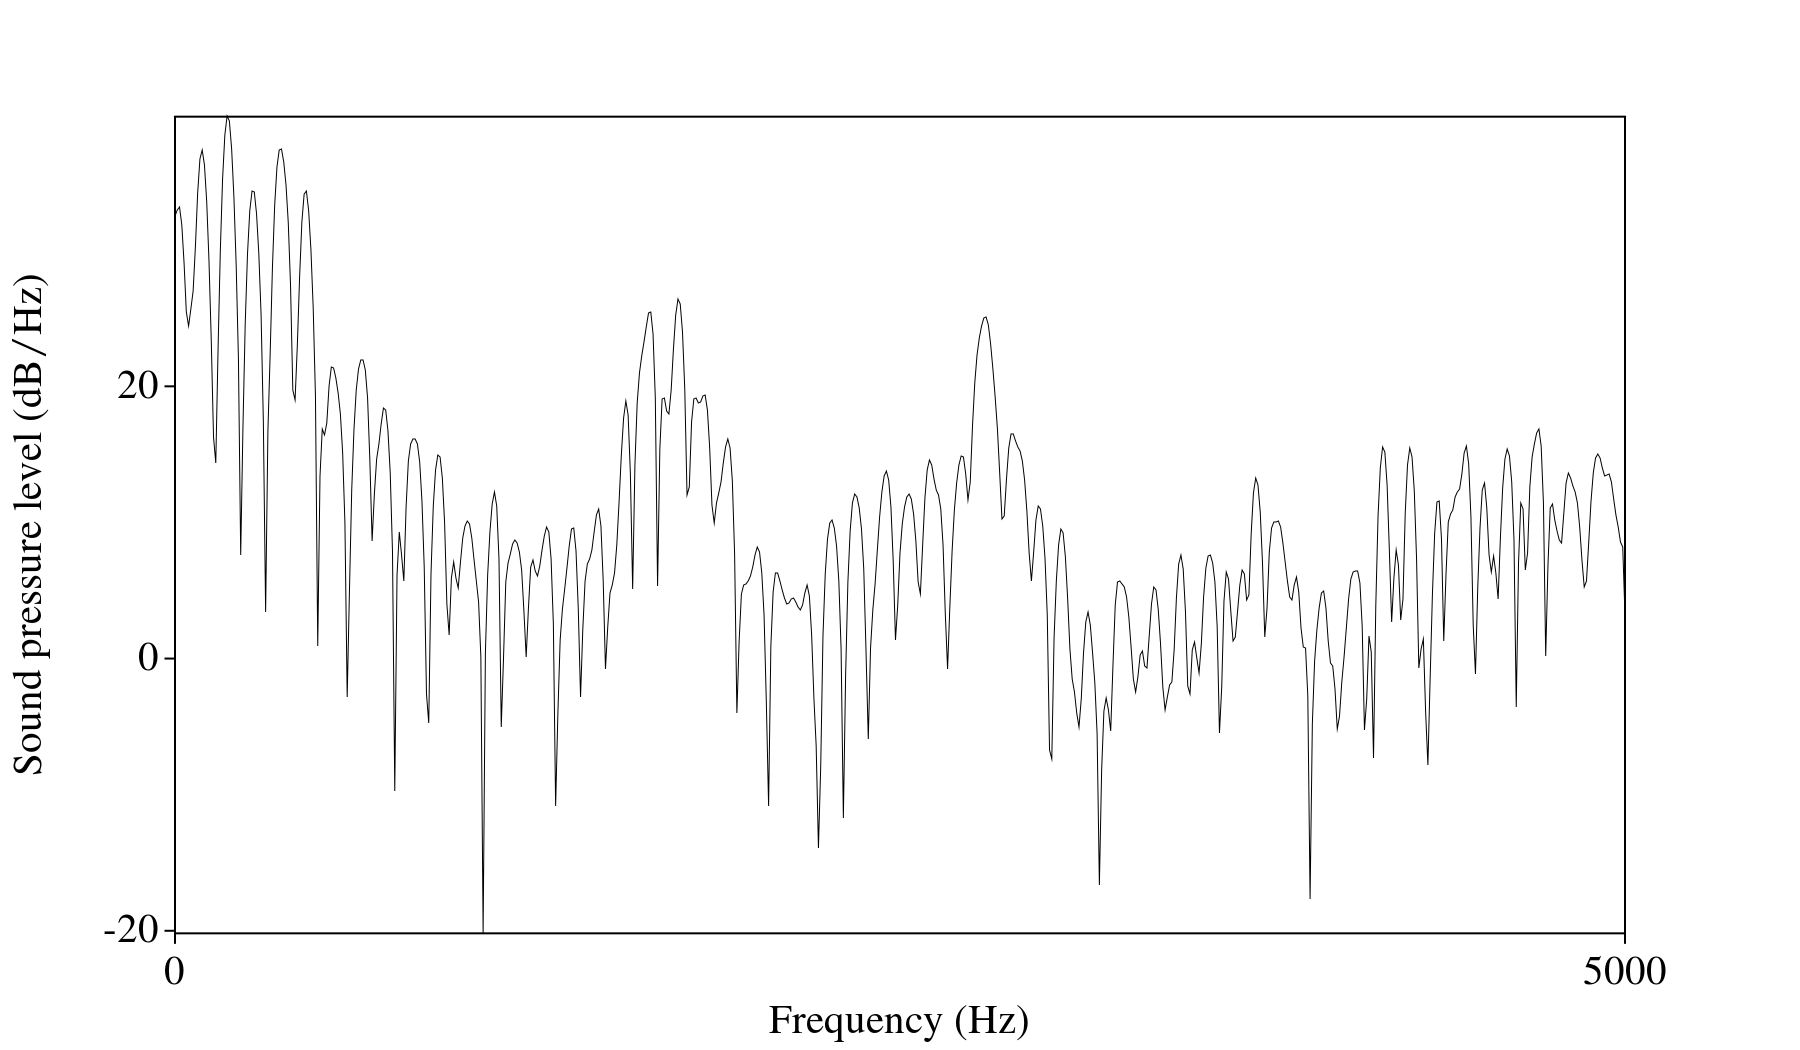
\includegraphics[width=0.5\textwidth]{figure/spctrm5k.png}
  \caption{Spectrum of the middle of an /I/ vowel.  Each ``hump'' is a separate ``band'' of frequency, called a harmonic.}
  \label{fig:spctrm5k}
\end{wrapfigure}
%
First, it is appropriate to review the acoustic structure of mouth emitted speech.  Speech could be divided into two primary categories - voiced and unvoiced.  Voiced speech is composed of bands of acoustic energy, called harmonics, located along a frequency spectrum (cf. fig \ref{fig:spctrm5k}).  
%
Certain harmonics will be dampened by the vocal tract, leaving others relatively unfiltered.  A region of harmonics containing more energy are called formants.  The location, shape, and transition over time of these formants (among other more minor features) are what encodes speech information for voiced sounds.  A spectrogram is a graph used to conveniently diagram the amplitude of various frequencies over time (cf. fig \ref{fig:spctgrm1k5k}).
%
\begin{figure}[h!]
\begin{subfigure}{0.95\textwidth}
  \centering
  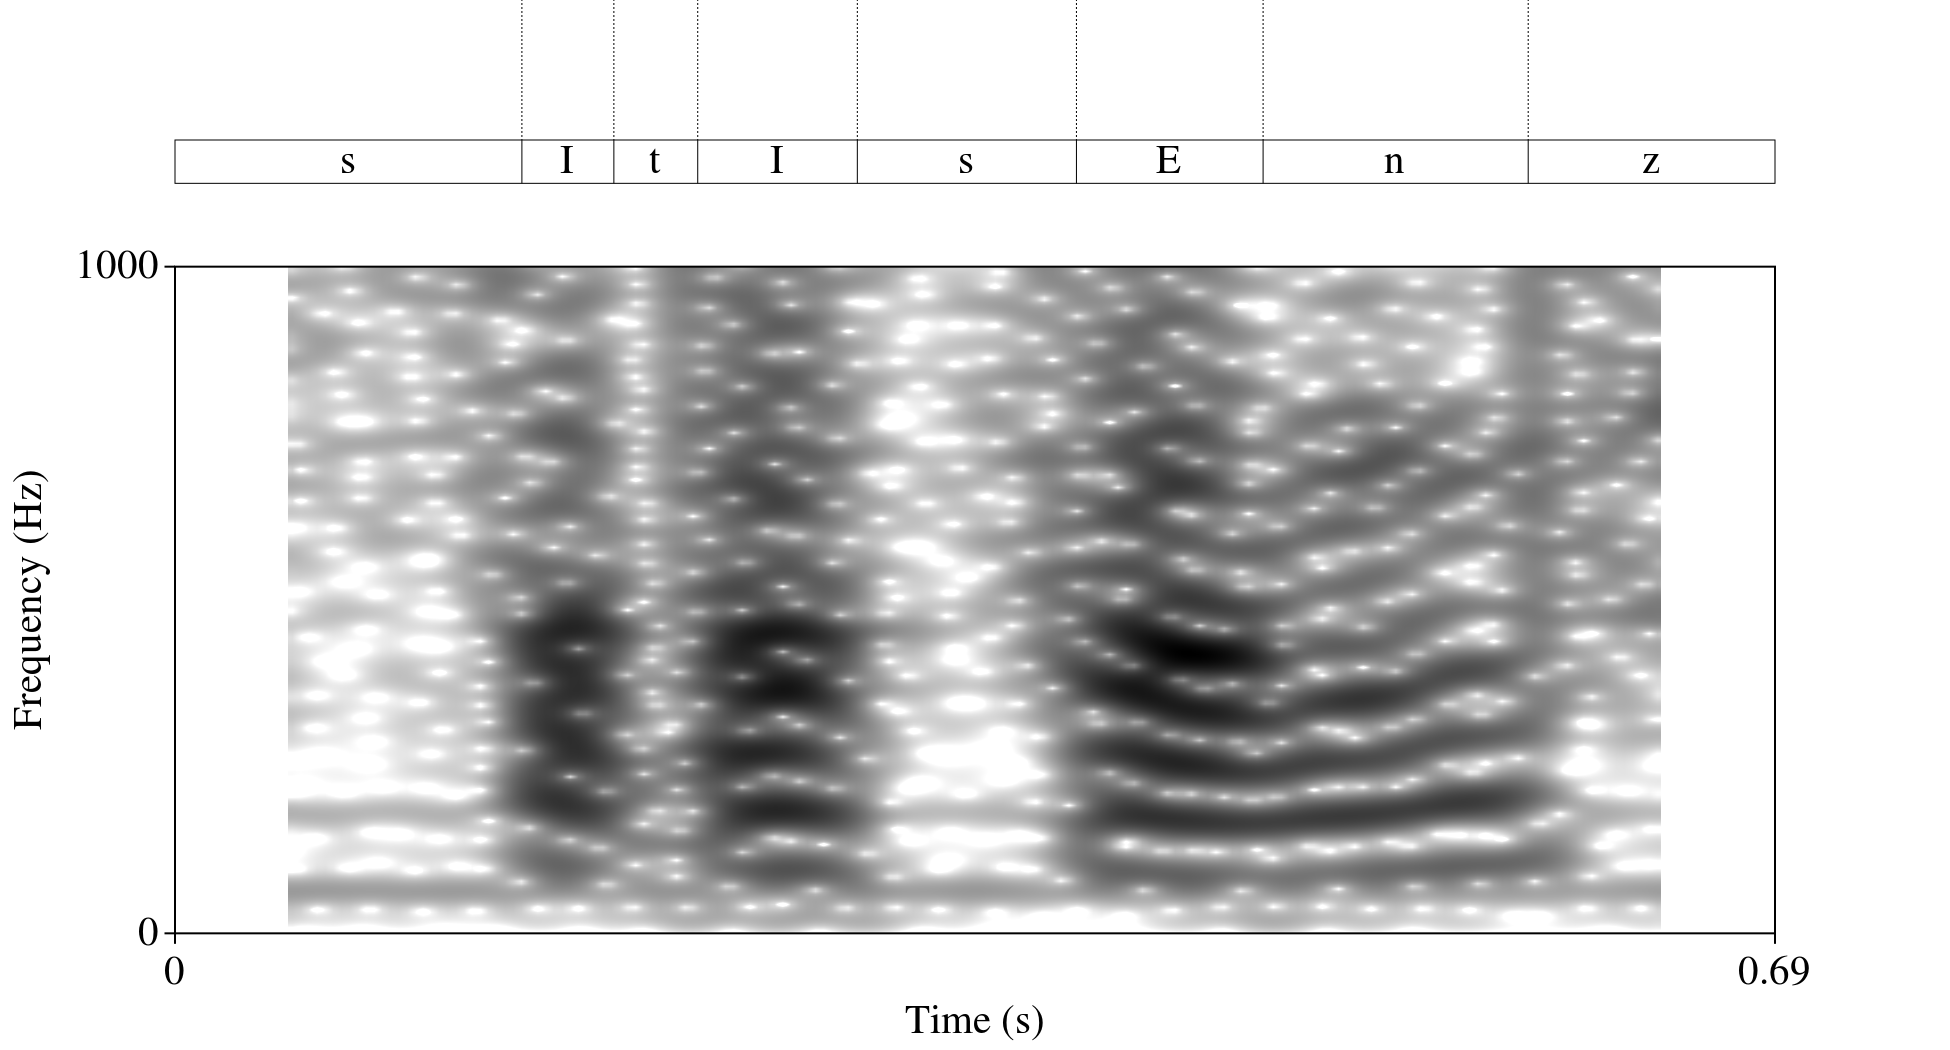
\includegraphics[width=0.95\textwidth]{figure/spctgrm1k.png}
  \caption{Zoomed to the 0-1kHz range for better visualization of harmonics.}
  \label{fig:spctgrm1k}
\end{subfigure}%
\hfill
\begin{subfigure}{0.95\textwidth}
  \centering
  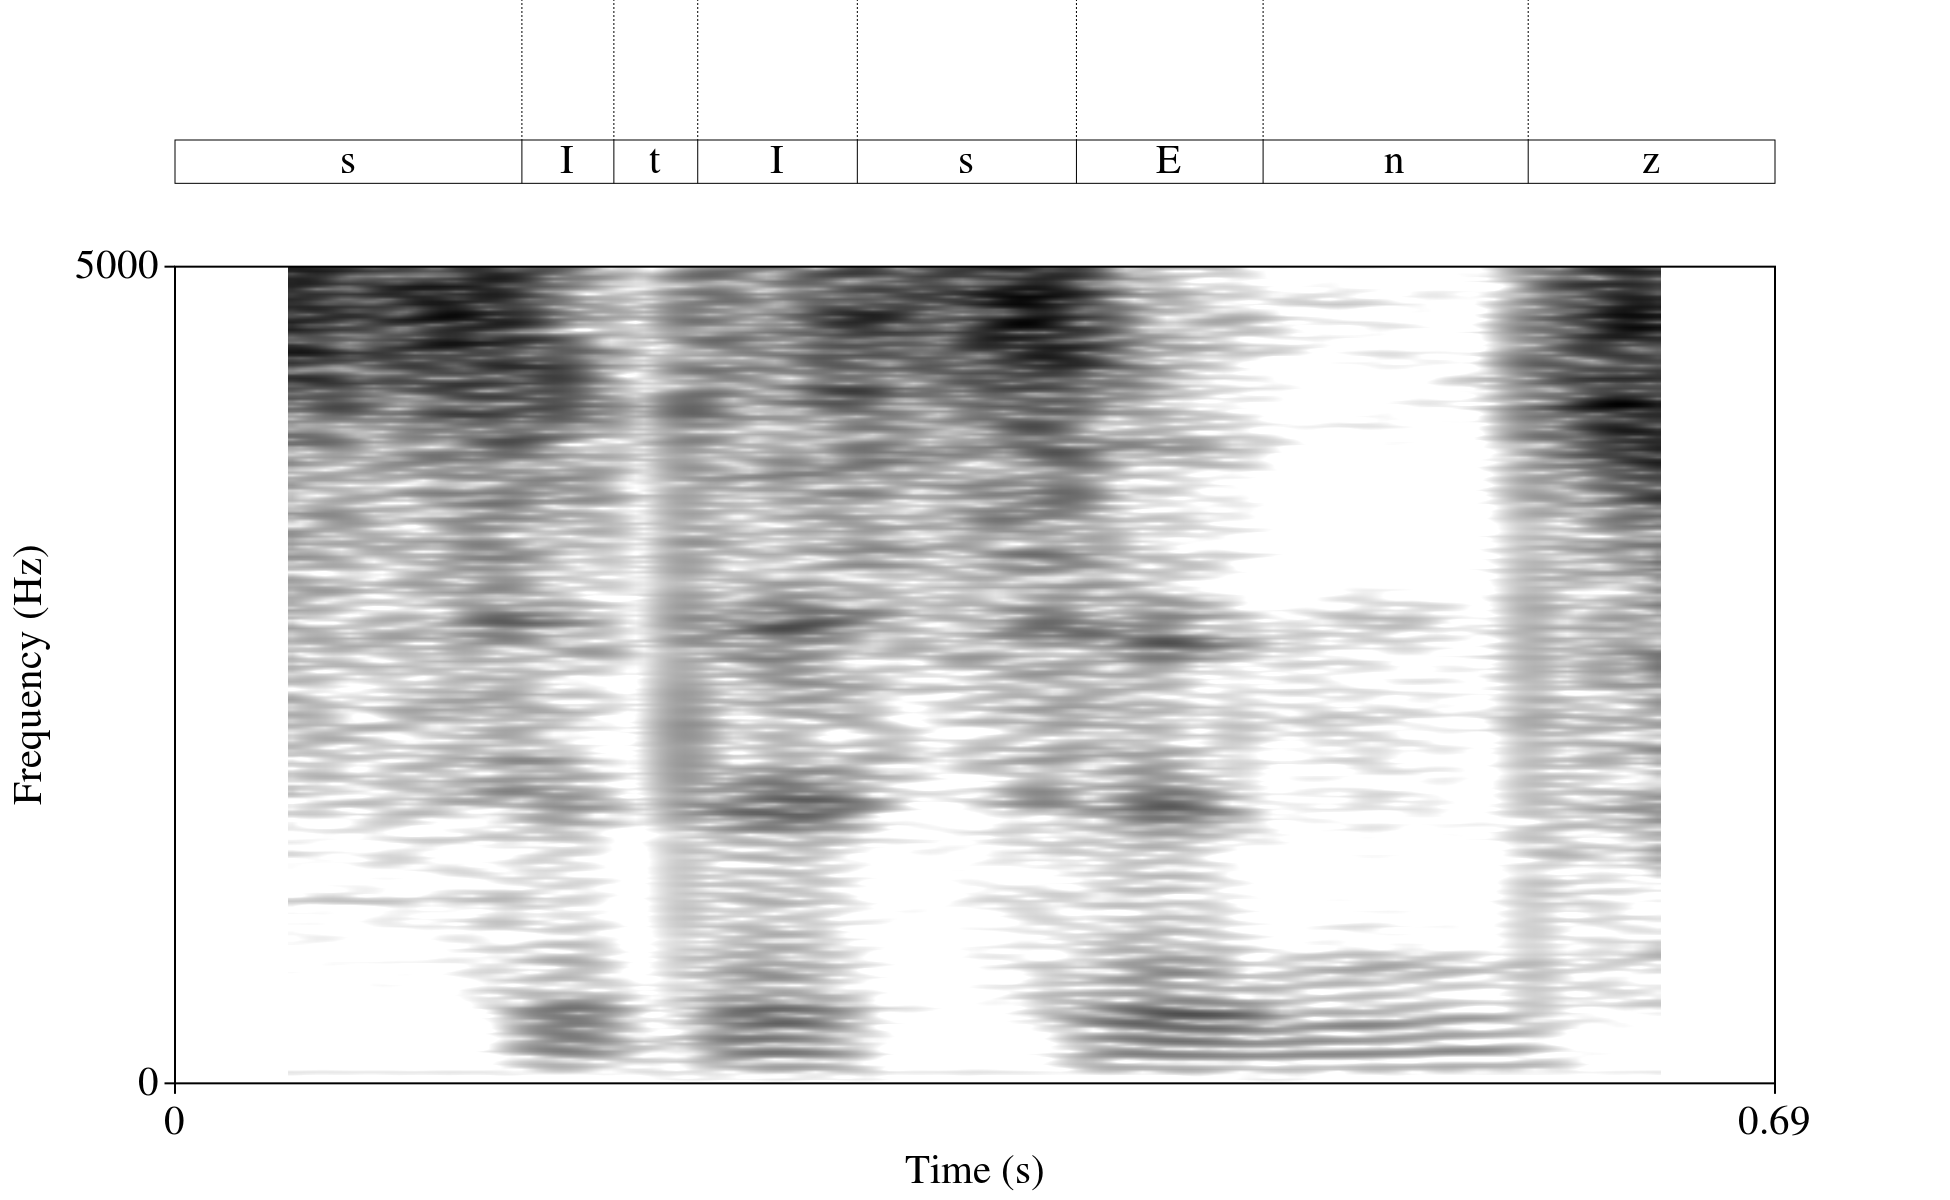
\includegraphics[width=0.95\textwidth]{figure/spctgrm5k.png}
  \caption{Zoomed to a more standard 0-5kHz range.}
  \label{fig:spctgrm5k}
\end{subfigure}
\caption{Spectrogram of the word ``citizen'' with phonetic transcription above.}
\label{fig:spctgrm1k5k}
\end{figure}

For unvoiced speech, the information used to recognize and categorize the speech sound is likely found in either the turbulent frication generally centered in higher frequencies cf. fig \ref{fig:spctgrm_s} (although some of the information can be found in lower frequencies), or found in the voiced information in the transitions into and out of the sound (\cite{story:10}).
%
\begin{wrapfigure}{l}{0.5\textwidth}
\centering
  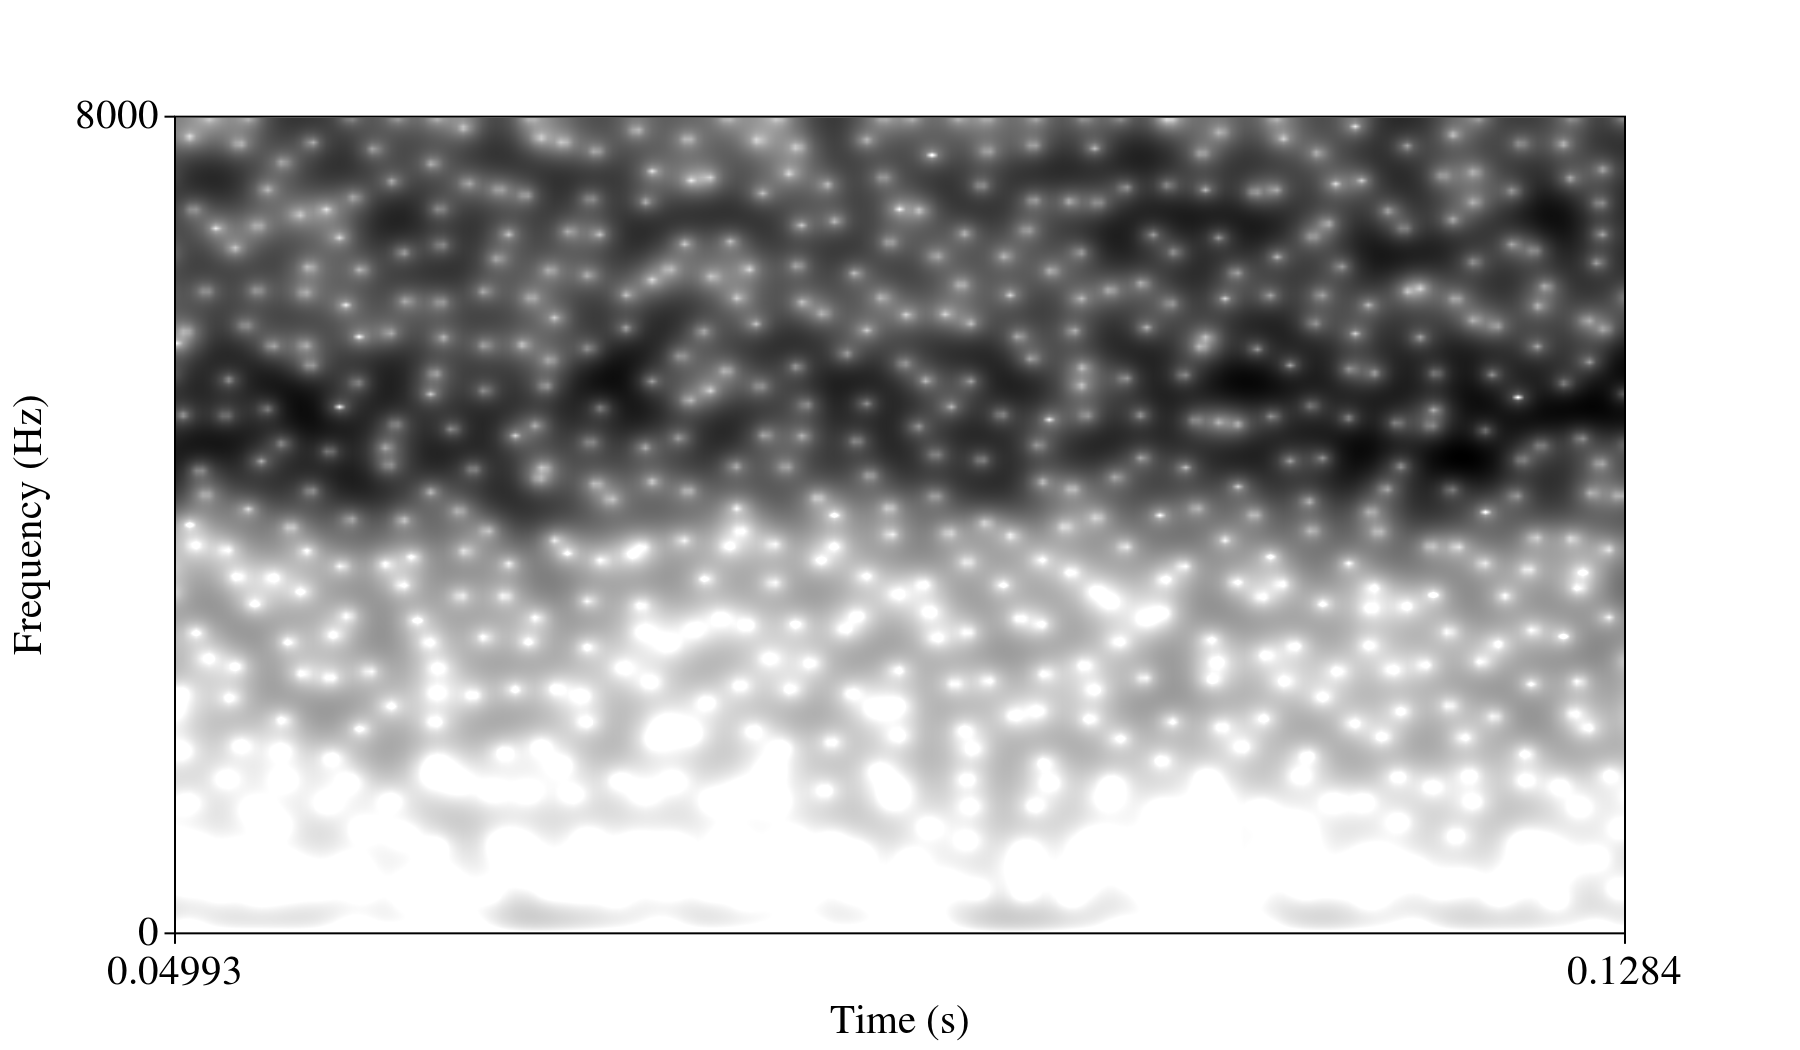
\includegraphics[width=0.5\textwidth]{figure/spctgrm_s.png}
  \caption{Spectrum of the initial /s/ in ``citizen''. Zoomed to range of 0-8kHz for visualization of high frequency energy.}
  \label{fig:spctgrm_s}
\end{wrapfigure}

% Discussion about Body/Bone conduction (mechanical)
\subsection{Bone Conduction}
Bone conduction of acoustic vibrations through a human head has been well studied (cf. \cite{allen:60}, \cite{hakansson:94}, \cite{stenfelt:00}, \cite{reinfeldt:10}, etc); however most of these studies have involved attaching a mechanical vibration device to an animal head or a cadaver skull, or using a vibrating piston on a live human participant, allowing for precise manipulation of the input signal.  
%The acoustic vibrations resulting from the mechanical device positioned on the head propagate to and are recorded by a recording device on a different location on the head.  
% Most of these studies, as well, are focused on audiometric bone conduction, i.e. the propagation of waves through the head and their effect specifically on the cochlea itself, which is not relevant to the present study.
% 
% %One study, \cite{hakansson}, used ``Live'' human subjects .  Titanium implants (pre-existing) for bone-conduction hearing aids anchored in the temporal bone behind the ear were used as the stimulation point for the mechanical vibrators.
% However, some do contain important findings about the general transmission of vibrations through a skull.
% Many of the early studies which were performed on cats do show that the sound generated by bone conduction propagating into the ear canal is dominated by low-frequency noise (\cite{tonndorf:72}).  Normally, the open ear acts as a high pass filter, dampening these lower frequencies passing into it via bone conduction.  When occluded, this filter is non existent, and the lower frequencies are more noticeably present (discussed in depth further below). 
%
% Other more recent studies on human subjects have agreed with these findings.  It has also been found that the acoustic response differs significantly depending on the location of the skull that is stimulated\footnote{Typically in these studies it is either the frontal bone or the mastoid process (\cite{bekesy:60}).}.
A few (cf. \cite{bekesy:48}, \cite{hansen:97b}, \cite{porschmann:00}, and \cite{reinfeldt:10}) have investigated body conduction when the source of vibration (i.e. sound) is a person's own voice, not an artificial mechanical vibrator.  These studies also record from the person's ear canal, and not another sensor on a different side of the skull.

The many studies that use a mechanical vibrator as a stimulus do so in part because using speech as a source is inherently messy.  This is so since speech 
\begin{enumerate*}[label={\alph*)}]
  \item  is not as easily manipulated as a simple mechanical vibrator,
  \item  contains far more frequency components than a simple mechanical vibrator, and 
  \item  takes multiple pathways to get to the ear: from the vocal chords, through tissue, and into the ear canal, and also from vibrations in the air all along the vocal tract\footnote{The speech sound is also filtered differently as it passes along the vocal tract}, through the solid medium of the head\footnote{Although, of course, the head is composed of different tissues with different densities and acoustic resonances}, and back into the medium of air inside the ear canal.
\end{enumerate*}
% 
\begin{wrapfigure}{l}{0.5\textwidth}
%\begin{figure}
\centering
  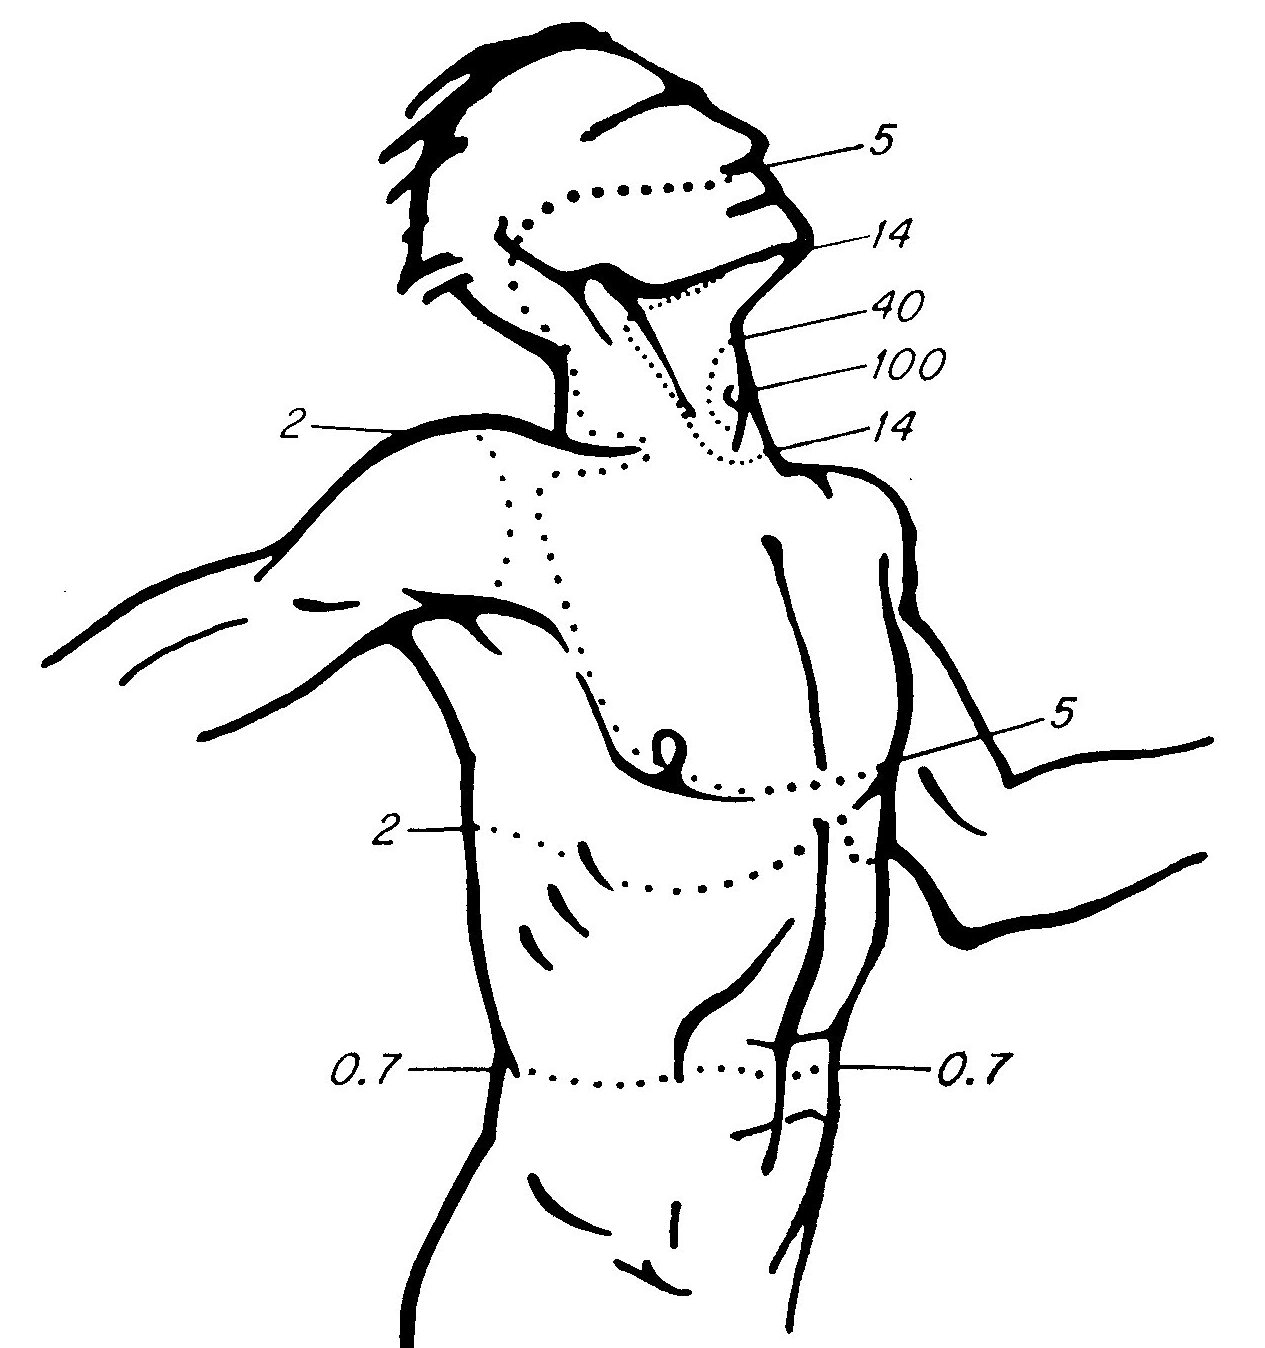
\includegraphics[width=0.5\textwidth]{figure/bekesy60-3b.png}
  \caption{Diagram of the propagation of speech waves throughout the body. Numbers correspond to percentage of the original amplitude of the speech remaining when reaching the marked location. Taken from \cite{bekesy:60}.}
  \label{fig:bekesyBodyTransfer}
%\end{figure}
\end{wrapfigure}
%
On top of this, the ear canal itself acts as a resonating chamber (\cite{rosen:91}), altering the signal beyond the distortion already caused by the passage through tissue and bone.  


\subsection{Peripheral Auditory System Anatomy}

Prior to discussing the resonating characteristics of the ear canal, it is important to become familiar with the basic ear canal anatomy.  The peripheral auditory system is generally grouped into three primary categories, the outer ear, the middle ear, and the inner ear (cf. Figure \ref{fig:ear-anatomy}).  The outer ear includes the pinna, the ear canal tube, and the tympanic membrane (ie. the eardrum).  Air-transmitted vibrations (sound) enter the ear canal through the opening at the pinna.  These then travel along the canal to vibrate the tympanic membrane, which passes the energy to the middle ear.  The middle ear includes the ossicles within the middle ear cavity.  These are a series of very small bones that the vibrational energy travels along, until it is passed into the cochlea in the inner ear.

The inner ear is composed of the cochlea, the semicircular canals (and vestibule), and the auditory and vestibular nerves.  The semicircular canals, vestibule, and vestibular nerve don't play a part in audition (their primary function regards balance sensitivity).  The cochlea receives the vibrations passed along through the middle ear ossicles.  These vibrations travel through a fluid substance in the cochlea, are sensed by hair cells within the cochlea, and transmitted as electrical pulses to the auditory nerve.

\begin{figure}[h]
\centering
  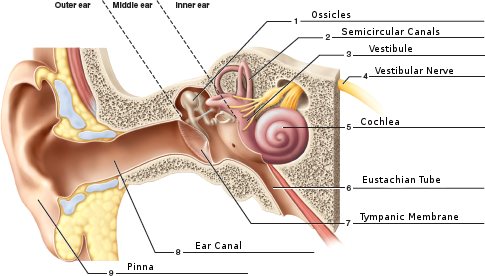
\includegraphics{figure/ear_anatomy.png}
  \caption{A diagram of the peripheral auditory system, including the outer ear, middle ear, and inner ear, up to the auditory nerve. (Image from \cite{martin:12})}
  \label{fig:ear-anatomy}
\end{figure}

Of interest to this present study is the outer ear.  Typically, as described above, vibrations will enter the ear canal through the opening at the pinna.  However, vibrations from one's own speech are also transmitted via the bone, cartilage, and tissue of the head.  Regardless of source, sound vibrations entering into the ear canal will be altered by the shape of the ear canal, described more below.

% Discussion about EAC resonance Theory
\subsection{Ear Canal Resonance}
% \begingroup
There has been much research on the resonating characteristics and amplitude response of the ear canal.  One such project was performed by \cite{stinson:89}, which studied fifteen human ear canals.  Their aim was to produce a model which can replicate the effect that the ear canal has on acoustics.
One challenge in producing such a model is the considerable variability in the shape of the canal - both between subjects as well as between the right and left ear canal of a single subject (\cite{stinson:89}).  These differences are apparent in curvature, length, volume, and cross-sectional diameter throughout the ear canal.  \cite{stinson:89} created silicon ear molds for each of the ear canals, which were used to generate three different computational models: one following the contours and dimensions of their ear molds exactly, another following the dimensions of the ear mold, but straightening contours and curvatures as if along a central axis, and the third as if the ear canal were a uniform tube with the same length and volume of the ear canal molds and previous models (see Fig. \ref{fig:eac_modelling}).  They noted that most significant differences between these models' spectral predictions of ear canal resonance occur above 6kHz.  
%
\begin{wrapfigure}{L}{0.5\textwidth}
\centering
  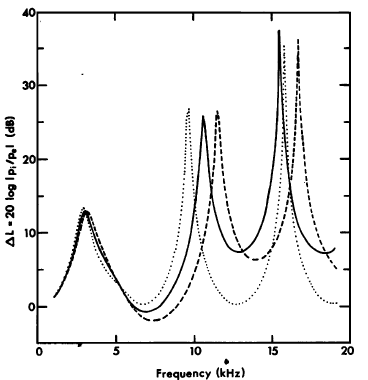
\includegraphics[width=0.4\textwidth]{figure/eac_mod_diffs.png}
  \caption{\cite{stinson:89} diagrams three different models of the ear canal resonance.  The bold line is based on their 3D canal molds from cadavers, the dashed line removes the curvature of the ear canal and acts as if the axis were straight, the dotted line assumes a constant diameter along a straight axis, with the same ear canal volume as the dashed and solid lines.}
  \label{fig:eac_modelling}
\end{wrapfigure}
%
Since much of the acoustic information for distinguishing speech sounds is located below 6kHz, several (cf. \cite{stinson:89,hansen:97b,stenfelt:07}) who have made efforts to model the ear canal, have chosen to simply treat it as if it were a uniform tube.  Treating the ear canal model as a uniform tube, as opposed to incorporating the nuances of its diameter and curvature, will not have much effect on the output of a model.

Another challenge is to obtain the dimensions of the ear canal needed in order to treat it as a uniform tube in the first place. Immittance measurements are widely used in audiology, and involve emitting a chirp or tone into a pressurized ear canal.  The chirp then bounces back from the tympanic membrane (assumed to have infinite impedance in a pressurized canal) and can be recorded (\cite{ballachanda:97}, 415): ``The sound pressure developed inside a rigid cavity from a known sound source is directly related to the volume of the cavity".  Therefore, the volume of the ear canal can be inferred for a subject using immittance testing without the need for invasive measurements (e.g. using a silicon mold).  Making an assumption about either an `average' diameter or an `average' length of the ear canal\footnote{The average length of the ear canal has been cited from 23mm (\cite{rosen:91}) up to approximately 29mm (\cite{stinson:89}) for a straight tube. The average diameter for the ear canal is approximately 7.1 mm (\cite{salvinelli:91}).}  would allow for the approximate calculation of the other dimension, given the measured volume. 
%These ear canal dimensions can then be plugged into any one of several models designed to approximate the ear canal dimensions.

\begin{figure}[h]
\centering
  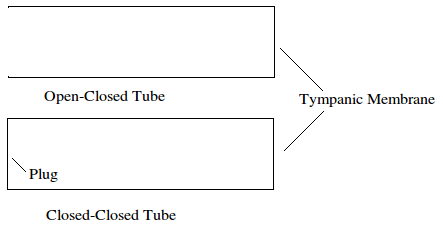
\includegraphics{figure/open-closed-tube.png}
  \caption{A diagram showing an example of an open-closed tube (top) and a closed-closed tube (bottom).  Applied to the case at hand, the closed end (on the right) in both figures would be the tympanic membrane.  The opening at the left (top) is the entrance to the ear canal, which can be plugged (bottom).}
  \label{fig:open-closed-tube}
\end{figure}

Once inside the ear canal with known approximate dimensions, it can either be modeled as an open-closed tube (if the ear is not plugged) or as a closed-closed tube (if the ear is plugged, cf. Figure \ref{fig:open-closed-tube}). This difference changes the resonance and reverberant structure of the ear canal.

%BC+EC-OE
\subsection{Ear Canal Resonance on Bone Conducted Speech}

There have been many studies, a few in particular (c.f. \cite{bekesy:48}, \cite{porschmann:00}, \cite{reinfeldt:10}) which use real human speech and measure the human ear as an open-closed tube.
%
The acoustics of uniform tubes is usually thought of in terms of an open-open tube, an open-closed tube, or a closed-closed tube.  Each of these have different resonating characteristics. The human vocal tract, for example, is normally modeled as an open-closed tube, where one end (the glottis) is generally considered ``closed'' for modelling purposes, and the other (the mouth) is generally considered to be ``open''.  Similarly, for the human ear, the tympanic membrane represents the ``closed'' end of the ear canal tube, and the ear canal opening at the concha, or pinna, is the ``open'' end (cf. Figure \ref{fig:open-closed-tube}).

\cite{porschmann:00}'s study is generally looking at the \textit{self-perception} of one's own voice, but in order to accomplish this devotes effort to looking at the bone conduction pathway separately.  A general 0.9 kHz resonance (with subsequent harmonic resonances) was found in the collected bone-conduction speech, with the amplitude gain generally present between 0.7 and 1.2 kHz.  This correlates with the 0.8-1.2 kHz range for the first resonance that others  (cf. \cite{hakansson:94}) have observed in mechanical-stimulated bone conduction studies. This would mean, in terms of speech, that one would expect to find higher amplitudes near the first formant.

However, in this study only two phones were used (/s/ and /z/), and a masking threshold\footnote{The masking threshold technique involves playing a pure tone at different frequencies and amplitudes while the participant is phonating. The participant indicates when the tone becomes audible over their own speech. Knowing the amplitude of the tone allows the researcher to know the amplitude of the speech as one becomes audible over the other. Having this knowledge, the spectrum of speech as it is perceived by the speaker can to be mapped.} technique was used to determine the frequency spectrum of the transfer function of body conduction.  This is admittedly a rather subjective method of determining the spectrum.  

\cite{reinfeldt:10}, on the other hand, use microphones to record the actual sound pressure level (SPL) of both air and body conducted speech. Furthermore, \cite{reinfeldt:10} used a more expansive and diverse set of phones.  While a resonance was found in generally the same frequency region for /s/ (and other phones) as that found by \cite{porschmann:00} (0.7 - 1.2 kHz), they discovered some interesting differences, which can be seen in Fig. \ref{BCrelAC}. Between each class that was used - voiceless sounds (/s/, /t/, /k/, and /tj/),  nasals (/m/ and /n/), and vowels (/i/, /e/, /a/, /o/) - a moderately similar frequency response is seen, yet there are some interesting distinctions to note (see Fig. \ref{BCrelACall}).

In particular, as can be seen in Fig. \ref{BCrelAC}, there is much inter-speaker variation within the body conduction of the same sound.  While it is difficult to track an individual speaker's relative spectral envelope within the figure, it appears that much of this difference, particularly in the lower frequencies, originates from a difference in amplitude, and not necessarily from different resonance locations along the frequency axis.  It is important to note that both Figs. \ref{BCrelAC} and \ref{BCrelACall} both contain \textit{relative} spectral envelopes - i.e. the difference between the air conducted and body conducted components of speech, and do not contain an absolute frequency spectrum of body conducted speech. 

An interesting observation is that the /e/ vowel has a relatively flat response up to 500 Hz, and only dips down to -5 dB around 1kHz.  Contrast this with the phone /s/, which below 500 Hz has a fairly high (yet falling) response, and only dips below -5 dB near 4 kHz.  However, compared with /e/, the body conducted to air conducted ratio for /s/ has a significant downward slope after 2000 Hz.  This is likely due to the fact that there is relatively little energy produced by /s/ in the low frequencies, allowing for a high ratio, which drops as the general energy of the phone increases.  This could indicate that most of the energy produced by a obstruent does not pass through to the ear canal (\cite{reinfeldt:10}).
% \begin{wrapfigure}{L}{1.1\textwidth}
\begin{figure}
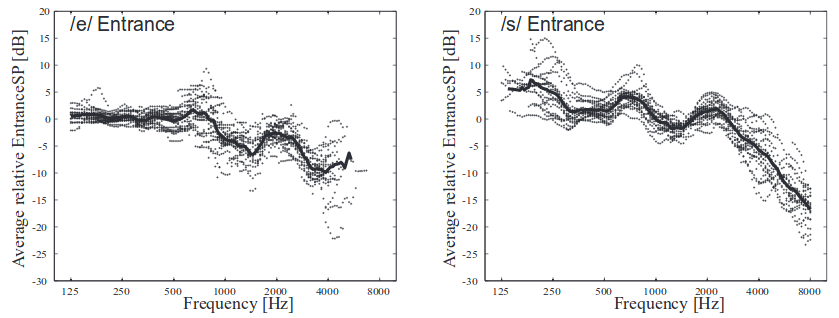
\includegraphics[width=1\textwidth]{figure/BCrelAC_e_s.png}
\caption{The amplitude of Body Conducted speech relative to the amplitude of Air Conducted  speech as recorded in the ear canal for the phones /e/ and /s/.  A value of less than zero indicates the amplitude of body conducted speech is less than that of air conducted speech, and a value greater than zero indicates a higher amplitude of body conducted speech than air conducted speech. The solid line indicates the mean, and the remaining data points are from individual speakers.  The signal was measured from the entrance of an open ear canal.  Taken from \cite{reinfeldt:10}.}
\label{BCrelAC}
\end{figure}
% \end{wrapfigure}

More specific dichotomies can be found between sounds within the same class. For example, the low vowel /a/ is pronounced with a more open mouth vs the relatively closed mouth of the high vowel /i/; consequently, the body conducted amplitude relative to the air conducted counterpart was much higher for /i/ than it was for /a/. An assumption could be made from the data that the more open the mouth is, the more energy is transferred to the air conducted signal (cf. Fig. \ref{BCrelACall}). \cite{reinfeldt:10}'s findings are backed by \cite{bekesy:60}, who also diagrammed the relative difference in amplitude in the ear canal between the air-conduction and body conduction of vowels (cf. Fig. \ref{bekesyPhoneDiff}), which also supports this hypothesis.  There was much inter-speaker variability, but it appears that the bone-conducted vowels with the least relative reduction in amplitude are the higher vowels.  Since the functions of other high sonorants (e.g. /u/) are not given, we cannot be certain if this is a phone-specific difference, or if it can be generalized to other sound with a [high] articulation in which the tongue is close to the roof of the mouth.  This would make sense, as the oral cavity is more ``closed'', trapping energy inside the cavity resulting in move reverberations passing through the head and into the ear canal.
%
\begin{wrapfigure}{l!}{0.5\textwidth}
% \begin{figure}
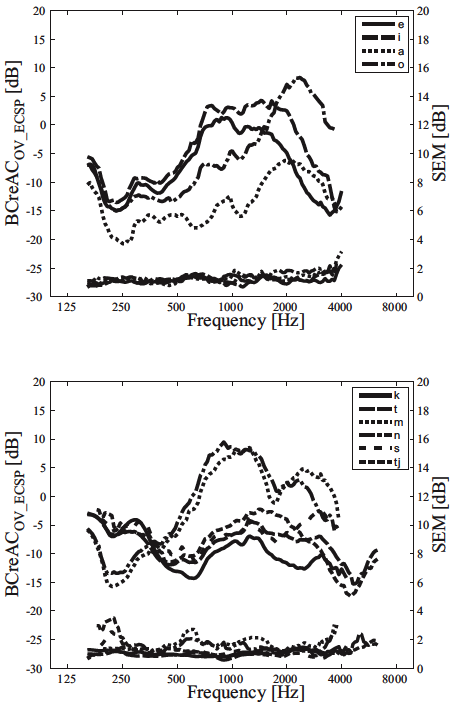
\includegraphics[width=0.45\textwidth]{figure/BC_rel_AC_all.png}
\caption{The mean relative amplitudes (left ordinate) of body conduction relative to air conduction for vowels (top plot) and other sounds (bottom plot).  The set of lines along the bottom of each plot represent the standard error from the mean (SEM), measure on the right ordinate.  Taken from \cite{reinfeldt:10}.}
\label{BCrelACall}
% \end{figure}
\end{wrapfigure}
%
On the surface, it appears, as well, that the more energy that is lost to air conduction during the production of low vowels (i.e. from a more ``open'' articulation), the less energy is transferred into the surrounding tissue.
%\footnote{\cite{bekesy:60} does not break down relative amplitude by frequency.}

Here it is important to re-emphasize that these transforms are given as body conducted amplitude \textit{relative to} air conducted amplitude for the given phone, and do not reflect the absolute air- and body-conducted amplitude of phones compared with one another.  For example, /a/ is a relatively loud air conducted sound due to its open articulation, and this loud air conducted component may cause its \textit{relative} body conducted component to appear quieter than the other vowels, when in reality it is possible that the body conducted component of both vowels have the same absolute amplitude.  Neither \cite{bekesy:60} nor \cite{reinfeldt:10} give information about body conducted components in relation to one another, and so a direct comparison between two bone-conducted phones cannot be conducted.


\begin{wrapfigure}{R}{0.5\textwidth}
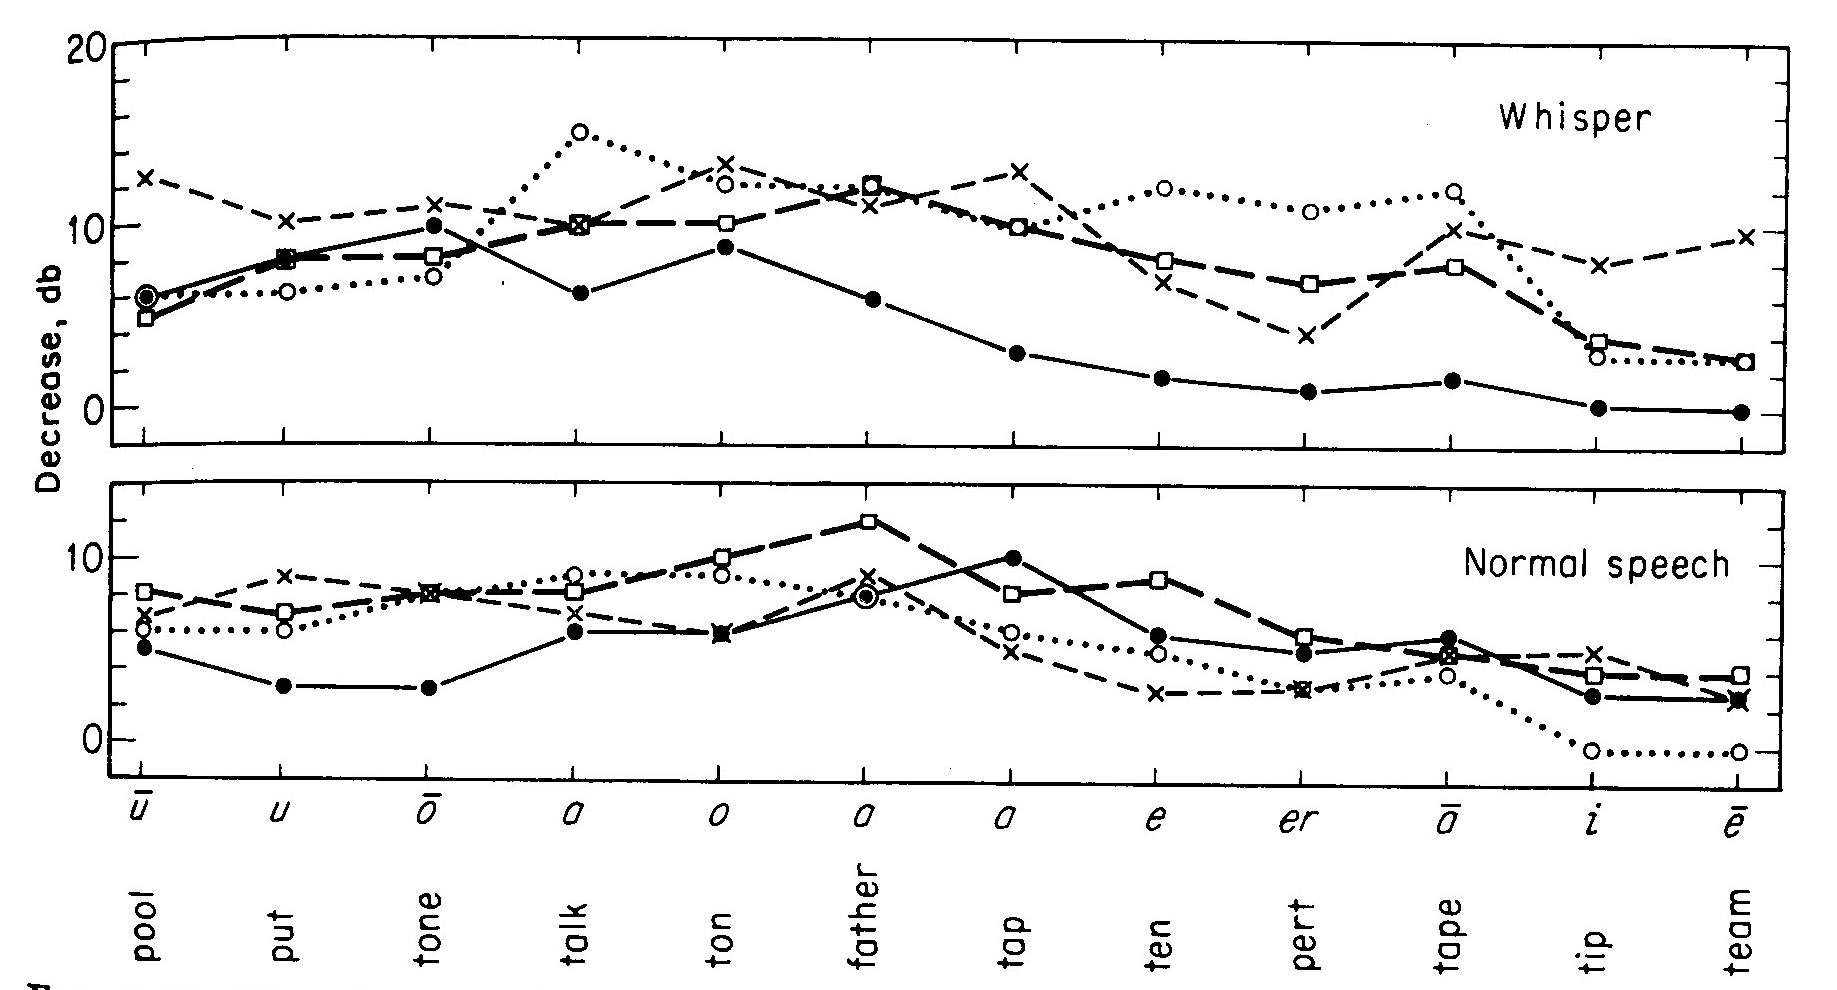
\includegraphics[width=0.5\textwidth]{figure/bekesy60-3.png}
\caption{Demonstrated the different effect on amplitude that closing the ear canal has on the different vowels of English.  Taken from \cite{bekesy:60}.}
\label{bekesyPhoneDiff}
\end{wrapfigure}

%BC+EC+OE% Discussion of the Occlusion Effect
\subsection{The Occlusion Effect on Bone Conducted Speech}

Returning to the notion of the acoustics and resonances of tubes, if the ear were to be occluded at its one open end, the ear canal would become - in effect - a closed-closed tube, and the frequency response would be altered accordingly.  This phenomenon, first noted by \cite{wheatstone:79}, is termed the occlusion effect (OE).  The occlusion effect\footnote{The occlusion effect is the change in sound pressure level (SPL) resulting from body conducted vibrations emanating into, and reverberating within, a \textit{closed} ear canal.} (OE) offers an amplitude gain to certain frequencies and dampens others.  This has been studied widely and extensively (cf. \cite{wheatstone:79,kelly:37,littler:52,goldstein:65}, among many others).  Generally, the occlusion effect (OE) results in a great increase in the amplitude of frequencies below 1-2kHz, acting as a low-frequency gain\footnote{This ``gain'' is a result of the transfer of energy from the higher frequencies} and that the amplitude of higher frequencies is dampened (as previously mentioned in the observation in studies of cats (\cite{tonndorf:72}).

%\cite{hansen:97b} and \cite{stenfelt:07} are primarily interested in modelling an occluded EAC, and this study requires the model to be a closed-closed tube - that of an \textit{occluded} ear. The models proposed by \cite{hansen:97b} and \cite{stenfelt:07} take many parameters, yet most can be considered to be either \textbf{too difficult to calculate frequently (- what does this mean? give an example)}, or relatively constant (e.g. the impedance of the middle ear, the speed of sound, etc.).  Both models, however, take the parameters for the length of the EAC, the average cross sectional area or diameter, and the volume of the EAC, which, are highly variable.

 
As with bone conduction in general, most of the research of the occlusion effect (OE) has been conducted using controlled mechanical vibrations.  \cite{bekesy:60} reports that when the ear canal is closed, there is an increase in amplitude within the canal from vibrations originating from a mechanical stimulus up to 2kHz, above which, vanishes quite suddenly (cf. Fig. \ref{fig:bekesyOEresponse}).

However, there is a variance in the OE - if using a mechanical vibrator - depending on the location of stimulation.  This difference is most present in the lower frequencies (\cite{dean:00}), where the relative amplitude increase (of body-conducted sound versus air-conducted sound) appears to be the greatest, but tends to wash out when slightly higher frequencies are reached\footnote{\cite{dean:00} found that the greatest relative amplitude increase occurs near 250 Hz, but the gain disappears when 1000 Hz is reached.}.  There are also differences based on the location of \textit{occlusion} within the ear canal, i.e. how deep a plug is placed in the ear canal. \cite{dean:00}'s results indicate this difference does not disappear as frequency increases; the relative amplitude increase is greatest with supra-aural earmuffs at lower frequencies, and lowest with deep inserted earplugs\footnote{\cite{dean:00} does not mention the explicit the depth for each condition, but from the article's description of the insertion procedure, it appears to be \~5mm.}. However, at 1 kHz, the shallow-inserted earplug has a greater relative amplitude gain than the supra-aural earmuff.

\cite{stenfelt:07} developed a model of an occluded ear using measurements generated from stimulating the skull separately at both the frontal bone and the mastoid process.
%
\begin{wrapfigure}{r!}{0.5\textwidth}
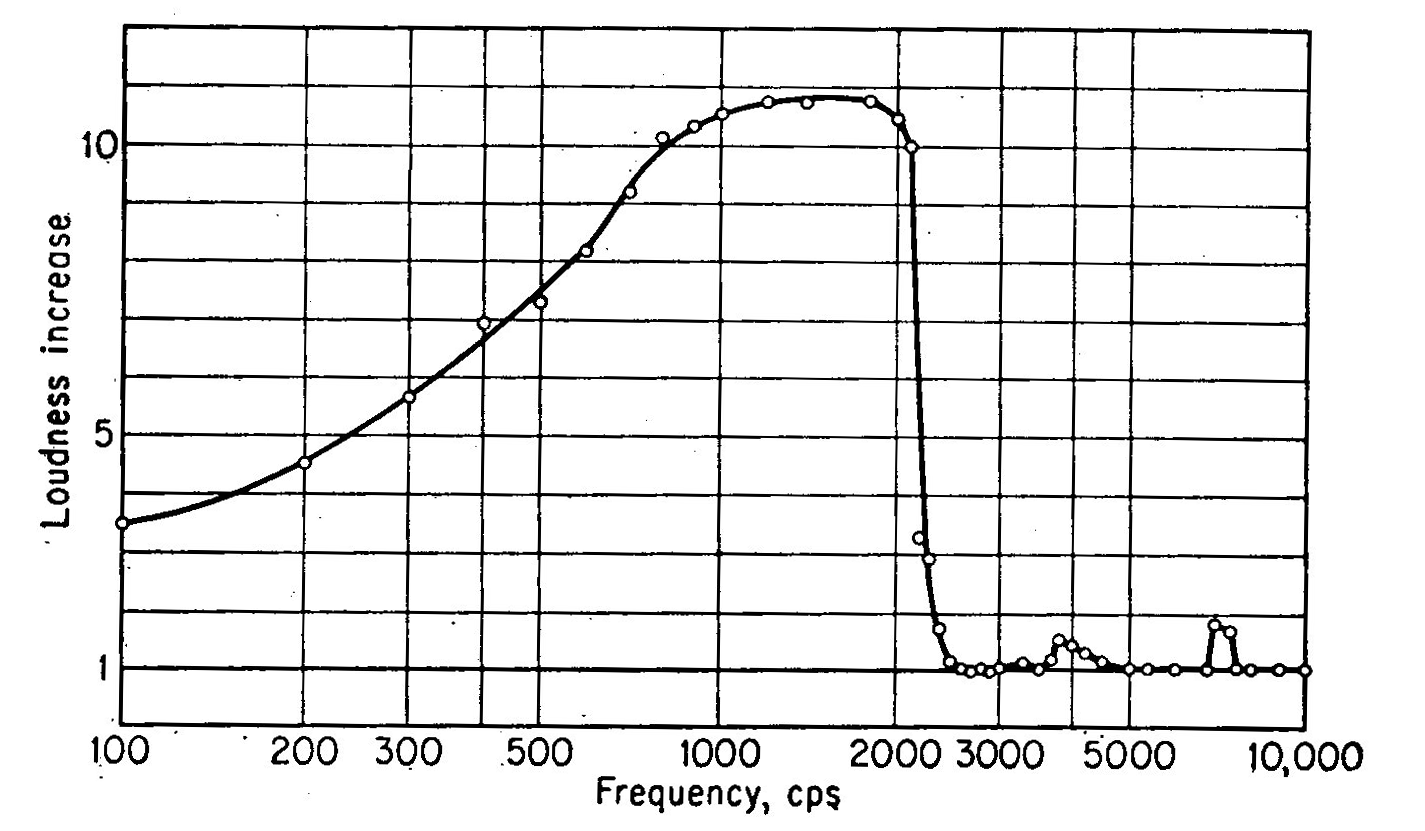
\includegraphics[width=0.5\textwidth]{figure/bekesy60-1.png}
\caption{The frequency response inside the ear canal when taking a mechanical vibrator to a participant's forehead.  Taken from \cite{bekesy:60}.}
\label{fig:bekesyOEresponse}
\end{wrapfigure}
%
Each site yielded a slightly different frequency response for the occlusion effect.  Stimulation at the mastoid generally resulted in a greater increase in very low frequencies below 1 kHz.  They also noted that the OE was greatest when using an ear plug near the opening of the ear canal, as opposed to supra-aural `ear muffs' or a deep-insertion ear plug, though an OE was noticeable in each condition; this is in direct contrast with \cite{dean:00}.   
%
\begin{wrapfigure}{r}{0.5\textwidth}
\begin{subfigure}{0.45\textwidth}
  \centering
  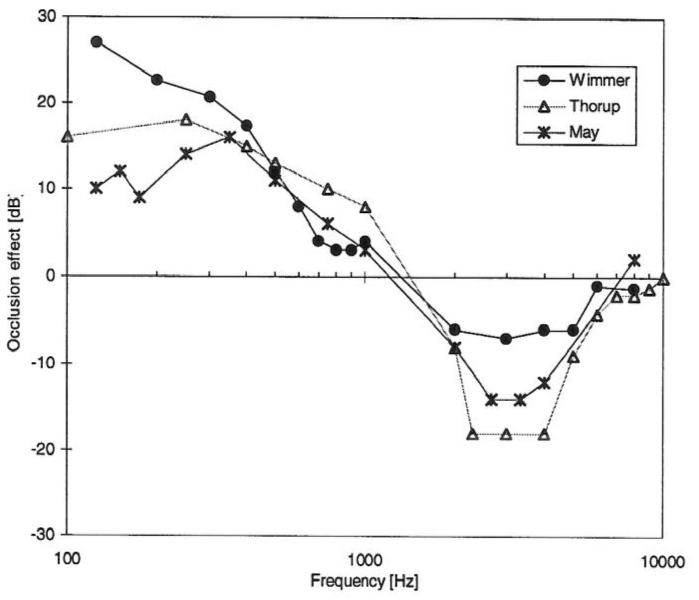
\includegraphics[width=0.8\textwidth]{figure/hansenAverageOE.png}
  \caption{ }
  \label{fig:hansenAverageOEa}
\end{subfigure}%
\hfill
\begin{subfigure}{0.5\textwidth}
  \begin{subfigure}{0.8\textwidth}
    \centering
    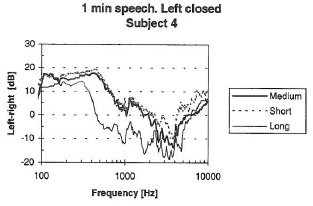
\includegraphics[width=1\textwidth]{figure/Hansen_OE-plot_a.png}
  \end{subfigure}
  \begin{subfigure}{0.8\textwidth}
    \centering
    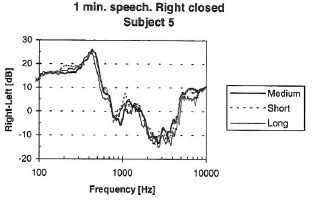
\includegraphics[width=1\textwidth]{figure/Hansen_OE-plot_b.png}
  \end{subfigure}
  \caption{ }
  \label{fig:hansenAverageOEb}
\end{subfigure}
\caption{In (a), three separate measured OE spectra. In (b), OE of two subjects with ear molds extending into the canal at different lengths (\cite{hansen:97b}).}
\label{fig:hansenAverageOE}
\end{wrapfigure}
%
\cite{dean:00} do not mention the size of earmuff used, but \cite{stenfelt:07} report the use of a large and small earmuff, with the latter providing a greater OE than the former, though both still below that of the shallow-insertion earplugs.

With shallow insertion, their model estimates a gain in amplitude of frequencies below 2 kHz, and dampening of those above; all insertion depths, according to their model, will at minimum, slightly dampen frequencies above 2 kHz.  As the plug is inserted deeper, the damping occurs on lower and lower frequencies. These results contrast slightly with \cite{bekesy:60}'s in Fig. \ref{fig:bekesyOEresponse} in that they predict higher, very low frequencies, as opposed with \cite{bekesy:60}'s bell-shaped resonance around 1-2kHz.


In contrast to the mechanical source studies above, \cite{hansen:97b} tested the OE using one's own voice as the input source.  \cite{hansen:97b} presents a graph comparing three spectra calculated from continuous speech from three separate publications\footnote{From \cite{wimmer:86}, \cite{thorup:96}, and \cite{may:92}} (Fig. \ref{fig:hansenAverageOEa}).  The study conducted its own tests (seen in Fig. \ref{fig:hansenAverageOEb}), which, by and large, agree with the previous studies.  
These represent the `average' effect of occlusion on speech, and appears to resemble other (mechanical-source) estimations.  \cite{hansen:97b} developed a model of the OE which largely agrees with these measurements.

The studies looking at human speech result in similar spectral resonances as those dealing with simple mechanical vibrations, except real-speech studies are able to capture the different OE for different kinds of complex sounds in a real speech environment, such as vowels.  



%% Allaying concerns of the effect of jaw movement on the occlusion effect.
While \cite{hansen:97b} found phone-specific differences in the occlusion effect (OE), it is ambiguous as to whether the differences are solely due to the differences in the transforms of phones as a result of body conduction (as seen in \cite{reinfeldt:10}), or if there are sound-specific differences introduced within the ear canal or by the occlusion effect itself.  
Some have posited that variability could critically stem from the placement of the jaw bone during speech next to the external auditory meatus, and as that changes as the jaw moves up and down\footnote{Thereby changing the impedance characteristics of the vibration of the mandible against the temporal bone housing the meatus (\cite{bekesy:60})} for `higher' or `lower' phones (e.g. /i/ vs /a/).  \cite{allen:60} studied the OE on participants with a unilateral resection of the mandible (one side of the jaw has been removed), and found essentially no distinction between the OE in either ear (i.e. with a mandibular joint adjacent to the cartilage of the ear canal or without).

Yet, \cite{hansen:97b}) found that a change in shape of the ear canal due to different jaw positions can create an acoustic ``leak" between the ear canal wall and the occlusion device; the occlusion effect, obviously, behaves differently when there are different sized ``leaks'' resulting in different levels of partial occlusion. 
\cite{hansen:97b} diagrams cross sections of the ear canal with the jaw at different positions; between a closed jaw and 5mm of opening, there is relatively little difference between the shapes of the ear canal.  Since \cite{borghese:97} found that the jaw moves relatively little vertical distance during actual speech (max opening approx. 6 mm), it can be assumed that the ear canal changes shape negligibly during normal speech with a snug-fitting occlusion device. 

In summary, it is important to emphasize the key difference between measurements from an open ear canal and those from an occluded ear canal, which can largely be seen between figs. \ref{BCrelACall} and \ref{fig:hansenAverageOEa}.  There is a massive increase in the amplitude of the lower frequencies, which is not present from an open-closed ear canal, and a sizable drop in amplitude after 2kHz, which similarly does not seem to manifest itself when the ear canal is not occluded.


%CONCLUSION
\subsection{Summary}

The aforementioned studies on body conduction and the occlusion effect, as would be expected, have indicated a fair deal of inter-person and inter-phoneme variability, and have shown the complexity involved in estimating the effect of body conduction and ear canal reverberance on speech entering the ear canal.  However, the transfer function from the vocal tract to the ear canal does have some standard characteristics, namely, the body and (occluded) ear canal act as a low-pass filter on speech, removing many of the higher frequencies which are within range of containing critical components for speech intelligibility.

%CONCLUSION to expt 1 lit review

%There is a possibility that the ear signal might be so low-pass filtered as to dampen the upper frequencies beyond retrieval and to the point that accurate recognition is unlikely.  In this case, there are still several possibilities, one of which will be outlined below.  

%While critical speech information may be lost, there is still critical speech information that will be present in the signal, namely the pitch.  The ear signal could be used to ``clean" a simultaneously recorded signal obtained from the mouth (which includes any ambient noise).  Since the occlusion effect acts as a gain in the low frequencies, the harmonic information of the voice signal can be reliably obtained from the ear signal.  Using this harmonic information, a comb filter (cf. \cite{nehorai:86}) could be developed and applied to the noisy mouth signal (cf. \cite{king:08}, \cite{cai:09}, \cite{jin:10}).  The comb filter acts as a series of narrow bandpass filters at equal (harmonic) intervals; when applied to speech, this can filter out the noise located in-between the harmonics.  

%There are a number of drawbacks with this method, however.  One is that this method primarily is used to recover voiced (harmonic) sounds, and fricatives or other voiceless sounds may not be able to be `cleaned'.  Another is that while speech is generally harmonic-like, it is not a perfectly harmonic signal, and there is a possibility that some of the higher harmonics might be accidentally filtered out.  This is particularly concerning as the higher frequencies are what is missing from the ear-recorded signal in the first place.


The methods described in this section, namely the models and transfer functions used by \cite{hansen:97b}, \cite{stenfelt:07}, and \cite{reinfeldt:10}, predict a general resonance within a closed ear canal that cause relatively higher amplitude in the lower frequencies (below 2 kHz), and a drop in frequencies above that range (with a few exceptions).  With this knowledge, it appears that it may be possible for recoverable speech information to be recorded from inside the ear canal.  While the skull will prevent much ambient noise from reaching a microphone placed in the ear canal, an occlusion device would need to be placed at the opening of the canal to aid in dampening the noise.  This occlusion results in the distortion described above.

This distortion is hypothesized to be, by and large, predictable (\cite{reinfeldt:10}), unlike ambient noise from the environment which is generally highly variable in both amplitude and form (\cite{zhang:17}).  Due to this, the technique of substituting potentially unanticipated, variable noise with the anticipated ``noise'' of body conduction and the occlusion effect allows for greater confidence that a usable signal could be recovered.  While the signal recorded is expected to be heavily low-pass filtered above approximately 2kHz and distorted, minor transformations, such as pre-emphasizing the higher frequencies, are hypothesized to recover some of the information that is lost, resulting in speech that will perform better than a noisy signal collected at the mouth in both ASR and human speech perception tasks.  

Section \ref{expt1} below describes the specific methods used to collect speech data from the mouth and the ear canal, and the analysis of the collected speech in an attempt to recover an intelligible signal with the knowledge outlined in this section.


\section{Experiment 1: Creating a dataset of ear-recorded speech\label{expt1}}

There are numerous constraints and requirement for the speech recordings required for this task, and it was necessary to create an original dataset for this study.  A small corpus is needed to be able to conduct ASR and Human speech perception experiments.  Primarily, a corpus needed to be created because there exists no known dataset of speech in which the recording location is inside the ear canal; speech recorded from this location is the primary focus of these studies.  Secondly, in order to be comparable, the speech at the ear, and the speech at the mouth, needed to be recorded at the same time, in the same conditions.  This was mainly to determine, when comparing the results of ear recorded and mouth recorded speech, whether the ear or mouth recorded speech performed better in the ASR and human speech perception tasks and to avoid potentially confounding variables that would occur if the two sets of speech were recorded separately. This is discussed further in subsection \ref{exp1design} below.

\subsection{Design}
\label{exp1design}
   
The goal of this experiment was to create a dataset of recordings, both from the mouth, in noisy conditions, and from inside the ear in the same conditions.  These recordings were needed to test the following (previously mentioned) hypotheses: (a) whether recording speech from the ear, external noise would be completely or largely eliminated, while simultaneously recorded speech from the mouth had a noisy background, (b) whether the speech from the ear was more intelligible and recognizable by an ASR system than noisy speech, and (c) whether the speech from the ear is more intelligible and recognizable by humans than noisy speech. 

In alignment with the CHiME challenge\footnote{The CHiME challenge tasks researchers to improve upon or surpass the performance of a baseline automatic speech recognizer used on noisy speech data.} guidelines, this study uses different types of background noise at different noise levels.  The noises used include the four sounds (bus, cafe, pedestrian area, \& street) from the \cite{chime:16}, plus a `factory' noise track.  A short portion of the audio with relatively level amplitude was extracted from each sound file to be played in the background.\footnote{Relatively level amplitude was used to allow for a more accurate comparison of the different SNR levels. Furthermore, if a sound file varied in amplitude, it would confound the recognition tasks as to whether a certain word is difficult to recognize, or the noise level that occurred at that portion in the sentence was a hindrance to accurate recognition. The exact portions of the sounds which were used are available online, along with the rest of the data at http://www.openslr.org/34/}

Many existing works in ASR and human speech recognition in noise use multiple SNR levels to demonstrate the effectiveness of the technique of noise removal (e.g. \cite{braun:16}).  This is generally done by adding a noise signal to already recorded clean speech, giving the researcher acute control over the SNR.  Due to the necessity of recording the noise while simultaneously recording the speech\footnote{This is needed to demonstrate the ability of the ear canal recording location to remove ambient noise.}, it was determined that noise would be played from a loudspeaker at pre-determined deciBel levels.  

Since human speech is variable in loudness, and amplitude will likely vary between and within speakers, only three, well-spaced noise levels were chosen to allow speakers' various `loudnesses' to fall in the same, broad categories.  Since conversational speech is generally around 70 dB, the noise levels chosen were 60 dB, 70 dB, and 80 dB\footnote{These were the `averaged' dB levels over the course of the sound file}. This would result in approximate SNR conditions of +10 (60 dB), 0 (70 dB), and -10 (80 dB)\footnote{As stated before, it is assumed that speakers will vary in how loud they speak, and so actual SNRs are expected to vary}.  +10 dB SNR is in the range of SNRs where ASR and human listeners have a very high recognition accuracy (cf. \cite{braun:16,gilbert:13}).  0 dB SNR occurs in a range in which ASR and human listeners are still able to make out most of a speech signal, but recognition begins to falter.  At -10 dB SNR, recognition performance very noticeably suffers.

80 dB was chosen as a max loudness, rather than a higher noise level to achieve a lower SNR, in order to leave a wide margin between it and any (albeit remote) possibility of hearing damage suffered by participants.  A `clean' (no noise) condition was also utilized for each sentence.  This creates 16 different conditions (5 noise types * 3 noise levels + 1 `clean' condition).  

\subsection{Stimuli}
Thirty sentences were chosen from 3 Harvard Sentence lists\footnote{The `Harvard Sentences' is comprised of 72 lists, each 10 sentences long, where each list of 10 sentences is phonetically balanced, where the proportion of each phone in the list corresponds with it's occurrence in the English language (\cite{harvardSents}).}.  These sentences were chosen due to being phonetically balanced (the distribution of phonemes in each list proportional to their occurrence in English), to their prolific use in speech science research, and specifically their history of serving as stimuli for many speech corpora (cf. \cite{kabal:02,hu:07}, the latter being a noisy speech corpus).  Lists 14, 28, and 57 were used, and chosen semi randomly, eliminating lists with potentially unfamiliar or rare words.  Each sentence occurs in all 16 conditions, resulting in 480 total stimuli.

  
\subsection{Equipment}

The experiment took place in a large soundbooth.  To create the artificially noisy environment a Yamaha MS101 III loudspeaker was hooked to an HP ProBook 6470b laptop.  A sound pressure level meter (SPL meter; Larson Davis Model 831) with a PCB Piezotronics Model 377B20 condenser microphone (omnidirectional) was placed 1 meter from the loudspeaker and measured the sound pressure to verify each of the three noise levels for each of the 5 noise types. A Grason-Stadler GSI Typstar Middle Ear Analyzer was used to measure the ear canal volume and test for plug leaks.  Two Countryman B2D directional lavalier microphones with fixed XLR connections were used to record the mouth speech and the ear speech.  These were hooked up to a PreSonus Digital Audio Firebox preamplifier, which was connected via TRS cables to a Zoom H6 Handy Recorder. A pair of 3M Professional Peltor Earmuffs with an noise reduction rating (NRR)) of -30 dB SPL were worn by the participant during the experiment.


\subsection{Participants}
Twenty participants were used in this study, ten female and ten male, all native speakers of American English with normal hearing.

\subsection{Procedure}

The participant was initially asked a few preliminary demographic questions\footnote{e.g. 2nd language (if any), etc. For a list of all information gathered, see Appendix A\ref{appendixB}.}. They were seated in front of the Middle Ear Analyzer.  An otoscope was used to ensure the right ear is mostly free of cerumen, to avoid blocking the microphone off from the rest of the canal and generally impacting the canal with cerumen.  The ear is fitted with an appropriate sized rubber clinical single-use ear tip, into which the Middle Ear Analyzer hose is already plugged.  An immittance test is performed, which involves playing a tone, and slightly and briefly pressurizing the ear.  The Middle Ear Analyzer checks that the ear plug solidly seals off the ear canal in order to be able to build up pressure and alerts the researcher to a leak if the plug is not securely in place.  This test gives an estimate of the volume in milliliters (mL) of the ear canal and of the middle ear, with precision to a tenth of a mL; additionally, a graph of middle ear function is given, which is checked for normalcy (cf. Appendix B\ref{appendixB}).  Several other measures are given which are not used in this study.

The distance from the end of the ear plug to where it is enclosed by the ear canal is measured to determine how far the plug was placed in the ear canal. %(cf. Fig. \ref{earplugInserted0.png} for diagram)
Since the length of the plug is known, this was done by placing a measuring rod against the cavity of the concha to measure how far the plug was sticking out of the ear, from which the insertion depth can be calculated. The decision to treat the cavity of the concha as the ``end" of the ear canal is taken from \cite{stenfelt:07}, who made molds of ear canals, and treated the rapid increase in volume (where the cavity of the concha begins) as the end to the ear canal.  This measure allows for the calculation of the depth of insertion of the earplug.

The Middle Ear Analyzer hose is then taken out of the ear plug - which is carefully left in place to ensure a continuous seal.  The participant then moves to a seat located in front of a computer monitor (cf. Fig \ref{fig:overallSetUp} for set-up diagram).  The participant is then instructed as to the proceedings of the rest of the experiment. One of the two microphones is taken, the wind-break foam removed, and is snugly inserted into the ear plug.  A mark on the microphone cable was used to ensure the end of the microphone was fully inserted to the end of the earplug.  There were several instances where the microphone was inserted deeper than, or just shy of, the end of the ear plug; the variance is within +/-1mm depth (cf. Appendix B\ref{appendixB}).  The earmuffs are placed over both ears.  Occasionally, a participant had glasses, or thick hair, which may have slightly compromised the seal.  A note was taken of this. 

\begin{wrapfigure}{R}{0.5\textwidth}
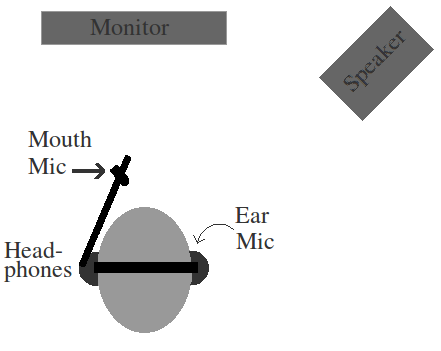
\includegraphics[width=0.5\textwidth]{figure/overallSetUp.png}
\caption{A diagram of the basic equipment set up for the experiment.  The in-ear microphone is placed under the headphones in the right ear.}
\label{fig:overallSetUp}
\end{wrapfigure}

A wooden rod was attached to the ear muffs, which extends forward, beside the participant's face.  The second microphone was attached to this wooden rod via the lavalier clip at the level of the participant's mouth.  The microphone was directed toward their mouth. % (cf. Fig \ref{microphoneDetailSetup2.png}).  
The placement of the microphone on the wooden rod was adjusted to be exactly 10cm away from the participant's infra-nasal depression.  At this point, the participant was asked to adjust the placement of their chair so that the microphone on the wooden rod was approximately 1 meter from the loudspeaker. Due to the length of the experiment ($~$45min), no effort was made to discourage minor shifting in body position.  The loudspeaker is on another table to the right of the participant, perpendicular to the direction of the microphone facing the mouth.

Both microphones were connected directly to the preamplifier through a fixed (non-changeable) XLR connection.  Both channels were set to the same gain on the preamplifier.  Two TRS cables took each microphone signal from the preamplifier to the recorder.  Both channels were adjusted to appropriate (different) gain levels on the recorder itself to achieve a similar loudness for both signals and prevent clipping.  These adjustments were made once the participant was situated, but before beginning the recording.

Once recording, an in-house computer program was used to display the stimuli sentences on a second monitor and play the background noises.  For each sentence, the participant saw the clean-condition (no noise) first.  The researcher was in the soundbooth with the participant listening through a pair of headphones connected to the preamplifier.  The participant was asked to repeat the sentence twice to get a rhythm for it, at a normal, conversational loudness, with a normal, declarative intonation.  The researcher asked the participant to repeat the sentence again in this condition if the rhythm or intonation of the two sentences did not match, or if the participant stumbled over a word.  Each of the following 15 iterations of the sentence (one for each noise-type/noise-level combination) the participant was instructed to speak only once.  If the rhythm of the sentence varied noticeably, or if a sentence was stumbled over, the researcher again asked the participant to repeat the sentence for that condition.  The sentences were not randomized, i.e. all 16 iterations of a sentence occurred consecutively\footnote{This was done to help the researcher ensure a similar intonation and rhythm for each iteration of the same sentence.}. Within each sentence group (after the `clean' condition, which always occurred first), all the noise conditions were randomized. Each stimulus is advanced by the researcher.

To help the participant notice when a sentence had been advanced\footnote{Wearing the ear muffs, they were often not aware when the noise condition changed.}, the number of the sentence condition was displayed underneath the stimulus (i.e. 1-16).  This had the unintended consequence of occasionally producing a mild list-intonation. 

After the recording was finished, the participant was asked to complete a short, 4 question questionnaire\footnote{cf. Appendix C\ref{appendixC} for exact (non-coded) and coded answers.} of their experiences during the experiment.  They were instructed to give as basic or as detailed answers as they wished, but to answer truthfully.  
%Extra credit in a Linguistics or other participating course was offered in exchange for participation in the experiment.

\section{Analysis of Collected Speech}

Each individual sentence was isolated in each recording with a Praat textgrid and extracted; this resulted in a sound file for each sentence, for each participant, for both the mouth-recorded and ear-recorded speech.  Figures \ref{spctgrmNarrowMouth_35}, \ref{spctgrmWideMouth_35}, \ref{spctgrmNarrowEar_35}, and \ref{spctgrmWideEar_35} show the narrow and wide band spectrograms for ear- and mouth-recorded speech from participant 35, a female, for a ``clean'' example of the sentence ``A cramp is no small danger on a swim''.  These two examples are fairly representative of the speech collected from each location.

\begin{figure}
\centering
\begin{subfigure}{.475\textwidth}
  \centering
  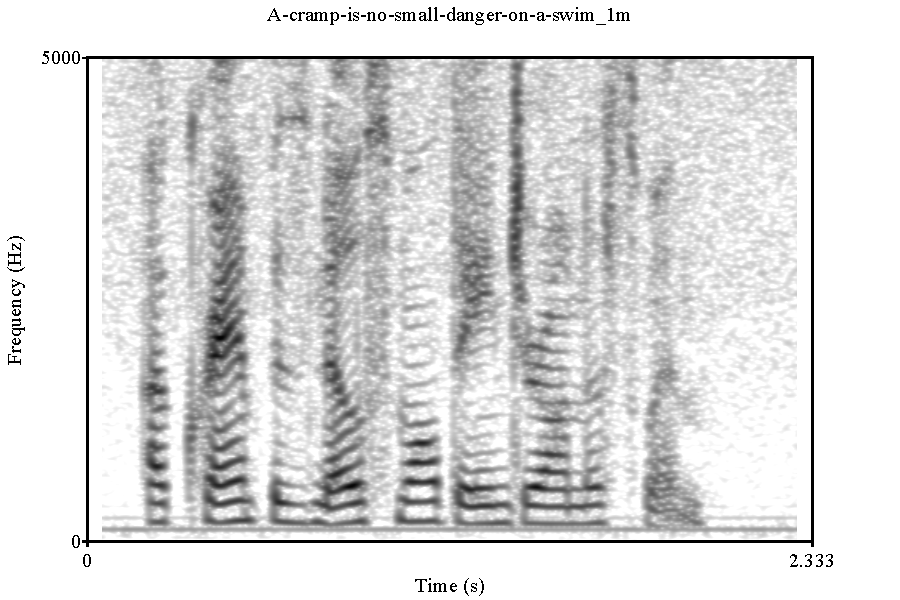
\includegraphics[width=1\linewidth]{figure/spctgrmNarrowMouth_35.pdf}
  \caption{Narrow band spectrogram of speech recorded at the mouth.}
  \label{spctgrmNarrowMouth_35}
\end{subfigure}%
\hfill
\begin{subfigure}{.475\textwidth}
  \centering
  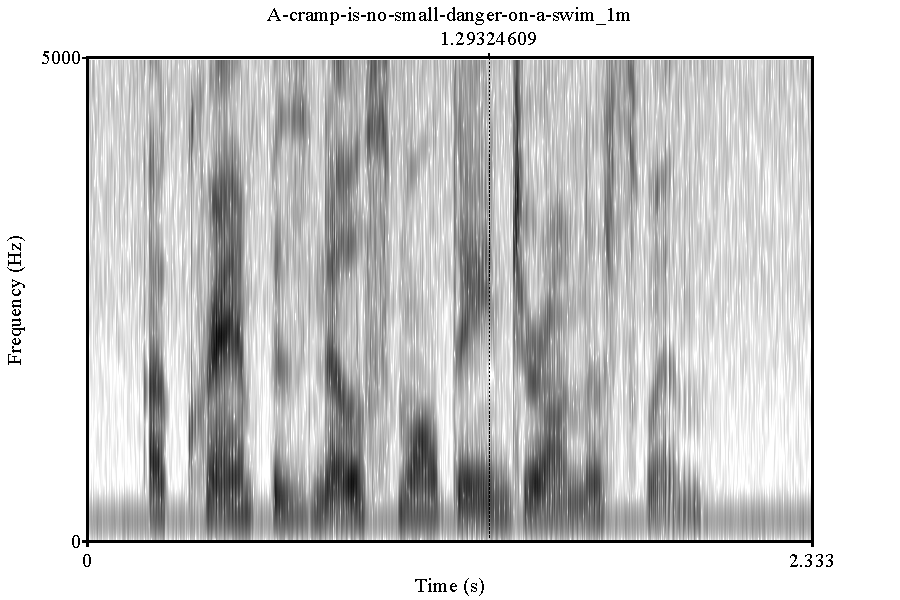
\includegraphics[width=1\linewidth]{figure/spctgrmWideMouth_35.pdf}
  \caption{Wide band spectrogram of speech recorded at the mouth.}
  \label{spctgrmWideMouth_35}
\end{subfigure}
\caption{Both (\ref{spctgrmNarrowMouth_35}) and (\ref{spctgrmWideMouth_35}) are the same sentence, ``A cramp is no small danger on a swim'', spoken by a female participant. This is the exact same sentence spoken at the exact same time as that in Fig. \ref{fig:spect_ear}.}
\label{fig:spect_mouth}
\end{figure}


\begin{figure}[b!]
\centering
\begin{subfigure}{0.475\textwidth}
  \centering
  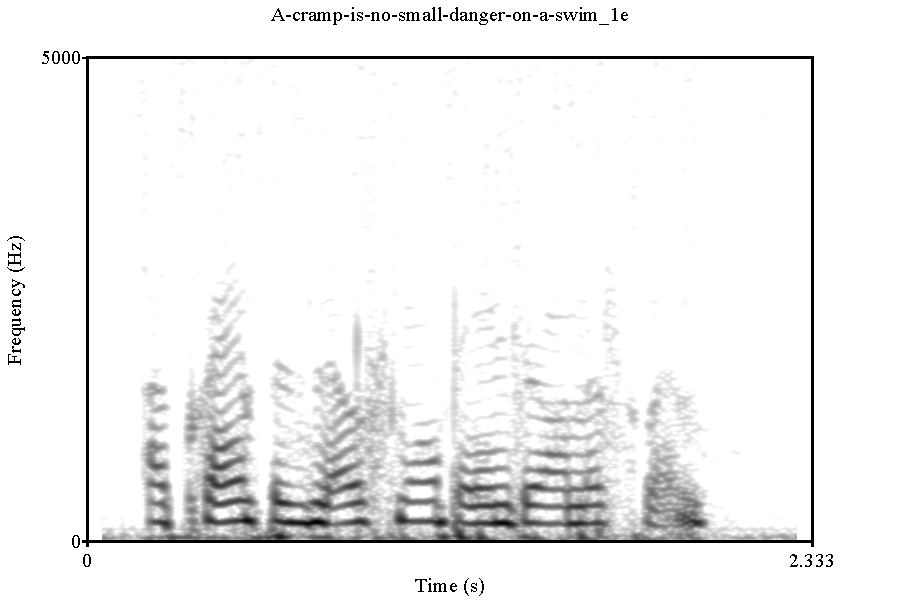
\includegraphics[width=1\linewidth]{figure/spctgrmNarrowEar_35.pdf}
  \caption{Narrow band spectrogram of speech recorded from inside the ear canal.}
  \label{spctgrmNarrowEar_35}
\end{subfigure}%
\hfill
\begin{subfigure}{0.475\textwidth}
  \centering
  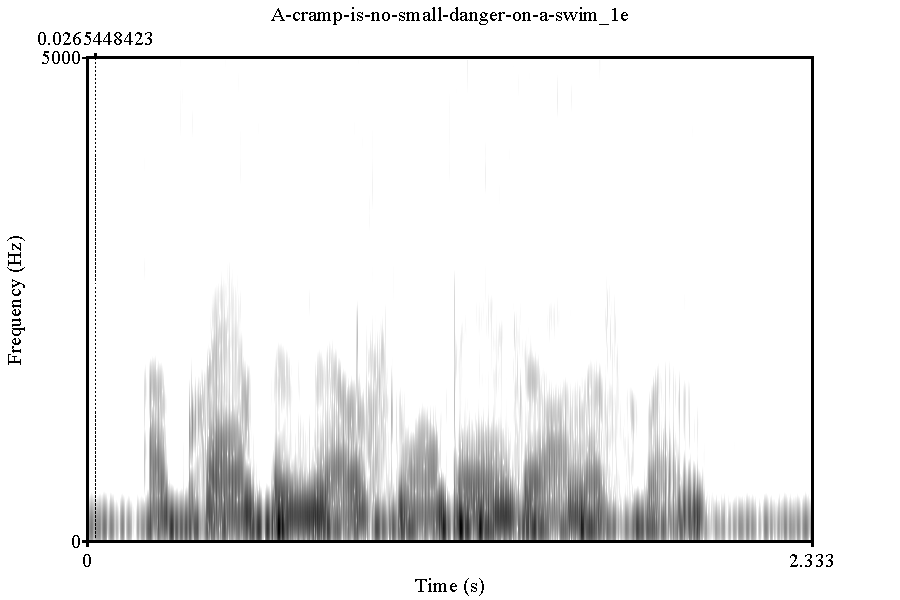
\includegraphics[width=1\linewidth]{figure/spctgrmWideEar_35.pdf}
  \caption{Wide band spectrogram of speech recorded from inside the ear canal.}
  \label{spctgrmWideEar_35}
\end{subfigure}
\caption{Both (\ref{spctgrmNarrowEar_35}) and (\ref{spctgrmWideEar_35}) are the same sentence, ``A cramp is no small danger on a swim'', spoken by a female participant. This is the exact same sentence spoken at the exact same time as that in Fig. \ref{fig:spect_mouth}.}
\label{fig:spect_ear}
\end{figure}


As can be seen, the speech collected at the ear is heavily low-pass filtered, and the mouth speech by itself has much more speech information.\footnote{It should be noted that while the two signals - from the mouth and from the ear - appear to have the same loudness, this is due only to the gain adjustment on the recording device during the experiment.  The speech from the ear was consistently \textit{louder} than the speech from the mouth; on a scale of 0-10, the ear microphone gain was normally set anywhere between 2 and 4, while the mouth microphone gain was normally set anywhere between 4 and 6.}
However, there are still clear harmonics in the existing range in the ear-recorded speech, and most of the lower two formants can also be seen.

When noise is present, it can be seen in Figs. \ref{spctgrmNarrowMouthNoise_35} and \ref{spctgrmNarrowEarNoise_35} that the noise does not affect the ear recorded signal nearly as much.  There appears to be some of the louder noise (seen in the mouth-recorded speech in Fig. \ref{spctgrmNarrowMouthNoise_35}) present in the upper frequencies of the ear recorded speech, but it is significantly dampened and the signal has an overall higher speech to noise ratio (SNR).

It should also be noted that the SNR in Fig. \ref{spctgrmNarrowMouthNoise_35} is much higher than originally intended.  For this particular example, the speech was recorded with an 80dB noise background, with the intent of obtaining a -10dB SNR.  Instead, the SNR for the sentence in Fig. \ref{spctgrmNarrowMouthNoise_35} is +6dB\footnote{The SNR was calculated by using background noises recorded in isolation in the soundbooth.  These were recorded at 60, 70, and 80 dB in the same soundbooth, with the same conditions and set up as a normal recording.  The noisy speech sound file was passed through a Hilbert Envelope, and a threshold was applied in order to extract just the speech data.  The RMS values of both the speech and raw noise vectors were calculated, averaged, and then used in the SNR calculation.  For explicit code, see Appendix E\ref{appendixE}}.  Unfortunately, this was widespread. This is attributed to a) the participant speaking louder than anticipated, resulting in a higher speech threshold, and b) the directionality of the microphone used eliminated much more background noise than anticipated.

\begin{figure}
\centering
\begin{subfigure}{0.475\textwidth}
  \centering
  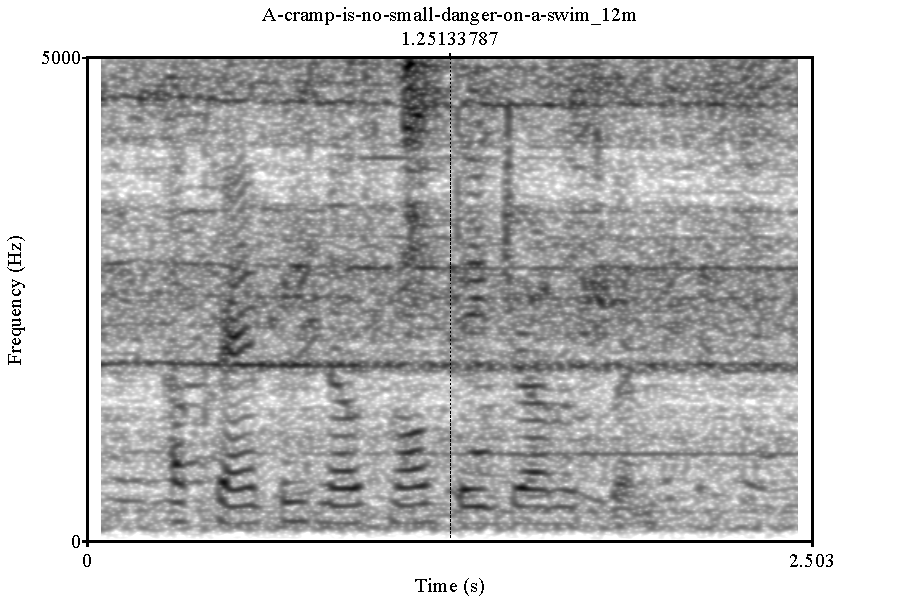
\includegraphics[width=1\linewidth]{figure/spctgrmNarrowMthNoise_35.pdf}
  \caption{Narrow band spectrogram of speech recorded at the mouth, with 80dB ``bus'' noise playing in the background.}
  \label{spctgrmNarrowMouthNoise_35}
\end{subfigure}%
\hfill
\begin{subfigure}{0.475\textwidth}
  \centering
  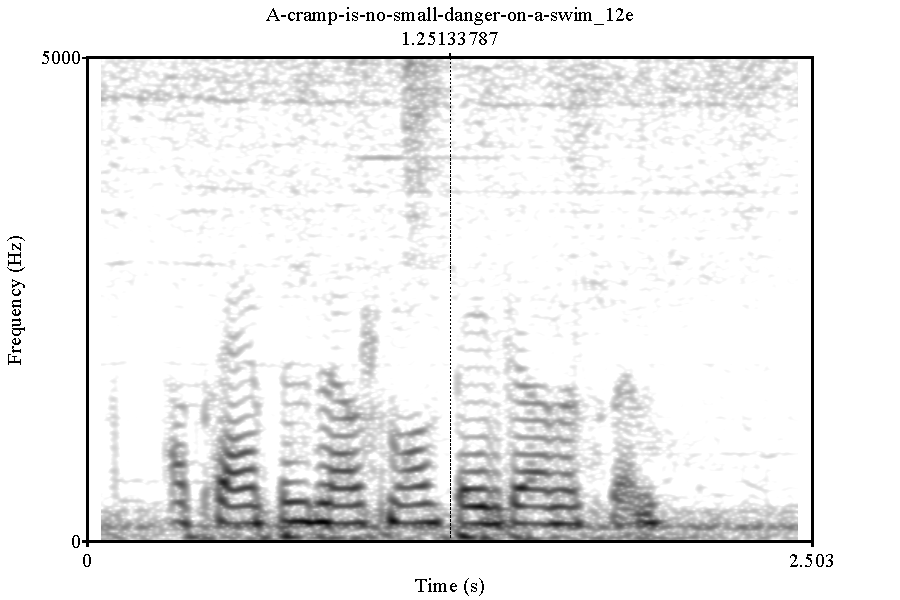
\includegraphics[width=1\linewidth]{figure/spctgrmNarrowEarNoise_35.pdf}
  \caption{Narrow band spectrogram of speech recorded inside the ear canal, with 80dB ``bus'' noise playing in the background.}
  \label{spctgrmNarrowEarNoise_35}
\end{subfigure}
\caption{Both \ref{spctgrmNarrowMouthNoise_35} and \ref{spctgrmNarrowEarNoise_35} were of the sentence ``A cramp is no small danger on a swim'', spoken by a female participant, recorded simultaneously.}
\label{fig:noise_mth_ear}
\end{figure}

In an attempt to see if there are recoverable frequencies in the higher ranges, the spectrogram range of ear signal was increased from 5kHz to 20kHz (see Fig. \ref{spctgrmEarNarrow20kHz}). There is certainly acoustic energy that makes it to the higher frequencies, but there do not appear to be harmonics, nor does any of the visible acoustic energy appear to correlate with the speech seen in the lower frequencies.
To be certain, the ear speech was pre-emphasized, seen in Fig. \ref{spctgrmNarrowEarNoisePremp_35}, which seems to confirm the lack of high-frequency speech information. 
\begin{figure}
\centering
\begin{subfigure}{0.475\textwidth}
  \centering
  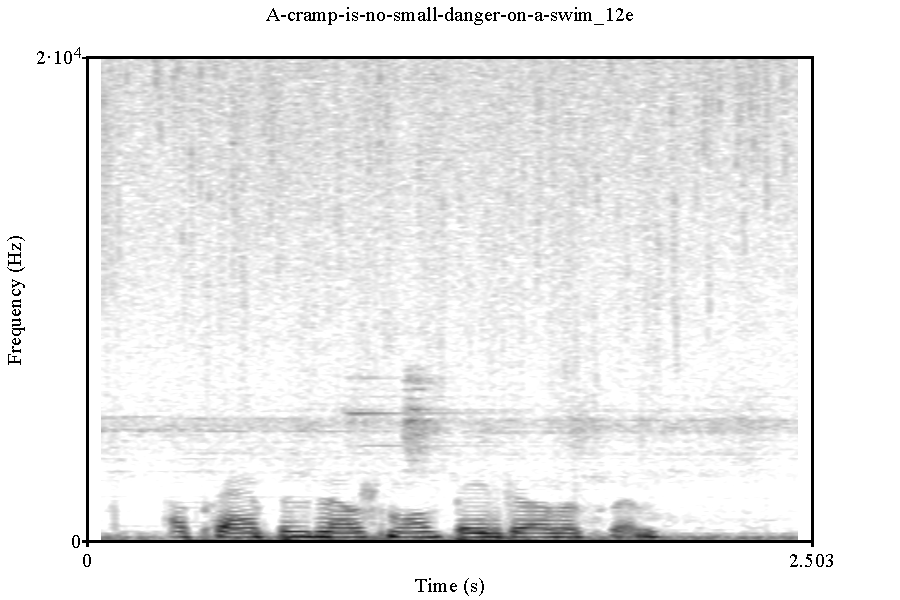
\includegraphics[width=1\linewidth]{figure/spctgrmEarNarrow20kHz.pdf}
  \caption{Narrow band spectrogram of ear recorded speech with 80dB ``bus'' background noise.}
  \label{spctgrmEarNarrow20kHz}
\end{subfigure}%
\hfill
\begin{subfigure}{0.475\textwidth}
  \centering
  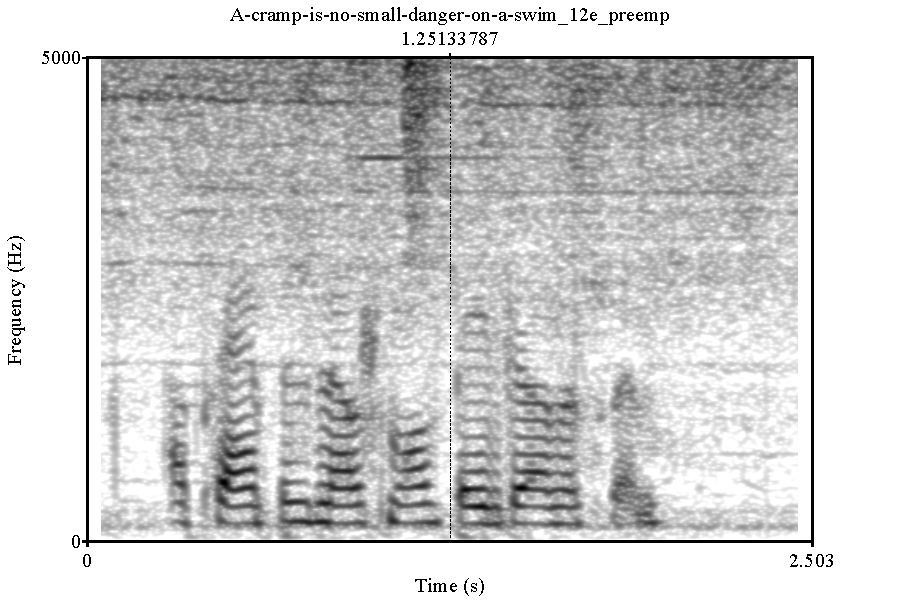
\includegraphics[width=1\linewidth]{figure/spctgrmNarrowEarNoisePremp.pdf}
  \caption{Narrow band spectrogram of ear recorded speech with 80dB ``bus'' noise.  The signal has been pre-emphasized.}
  \label{spctgrmNarrowEarNoisePremp_35}
\end{subfigure}
\caption{Narrow band spectrogram of ear-recorded speech from 0-20kHz to look for possible speech information in higher frequencies, of the sentence ``A cramp is no small danger on a swim'' spoken by a female participant. Note, the noise only extends to 8kHz.}
\end{figure}
\begin{figure}[b!]
\centering
\begin{subfigure}{0.475\textwidth}
  \centering
  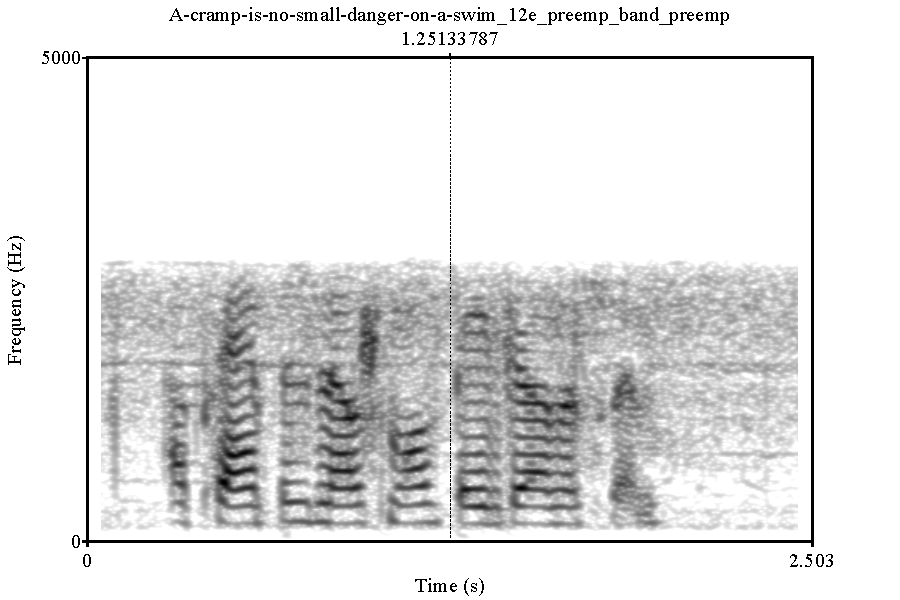
\includegraphics[width=1\linewidth]{figure/spctgrmNarrowEarNoisePrempFiltPremp.pdf}
  \caption{The ear recorded speech, pre-emphasized, filtered at 2500 Hz with 500Hz slope, and pre-emphasized again.}
  \label{spctgrmNarrowEarNoisePrempFiltPremp_35}
\end{subfigure}%
\hfill
\begin{subfigure}{0.475\textwidth}
  \centering
  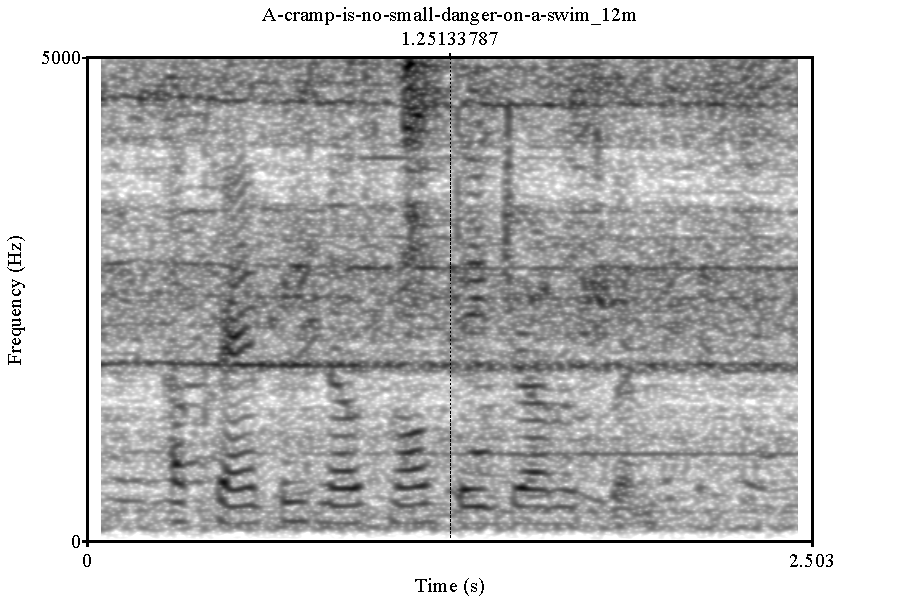
\includegraphics[width=1\linewidth]{figure/spctgrmNarrowMthNoise_35.pdf}
  \caption{The noisy spectrogram of the mouth-recorded speech; previously seen in \ref{spctgrmNarrowMouthNoise_35}, repeated here for ease of comparison.}
  \label{spctgrmNarrowMouthNoise_35_compare}
\end{subfigure}
\caption{Narrow band spectrogram of ``A cramp is no small danger on a swim'' recorded at the ear (\ref{spctgrmNarrowEarNoisePrempFiltPremp_35}) and the mouth (\ref{spctgrmNarrowMouthNoise_35_compare}) and spoken by a female participant, with 80dB bus noise in the background.}
\label{fig:ear_pfp}
\end{figure}
It appears that while those fainter harmonics in the lower mid-range frequencies have become more pronounced, there is no new speech information in the upper frequencies which has made it past the noise threshold.

This ear-recorded signal was then low-pass filtered at 2500 Hz with a 500 Hz smoothing slope. To further emphasize the higher frequencies in the available range (and to smooth over the 'muffled' attribute a bit), the sound was pre-emphasized a second time (after filtering).  This can be seen in Figure \ref{spctgrmNarrowEarNoisePrempFiltPremp_35}, next to the noisy mouth speech for comparison in Figure \ref{spctgrmNarrowMouthNoise_35_compare}.

\section{Discussion}

\subsection{Limitations}
\label{ch2:limitations}

During data collection, there were several issues that affected the data.  
The particular recorder which was used, when the gain knobs were turned up into the slightly higher range, would produce a low-frequency humming sound (cf. Figure \ref{fig:low_freq_hum}).  This was much more prominent for the mouth-recorded signals, as the gain for this channel was turned up higher.  Since the headphones the researcher was using were plugged into the preamplifier, this was not noticed until most participants were already recorded.

\begin{figure}[h]
\centering
\begin{subfigure}{0.475\textwidth}
  \centering
  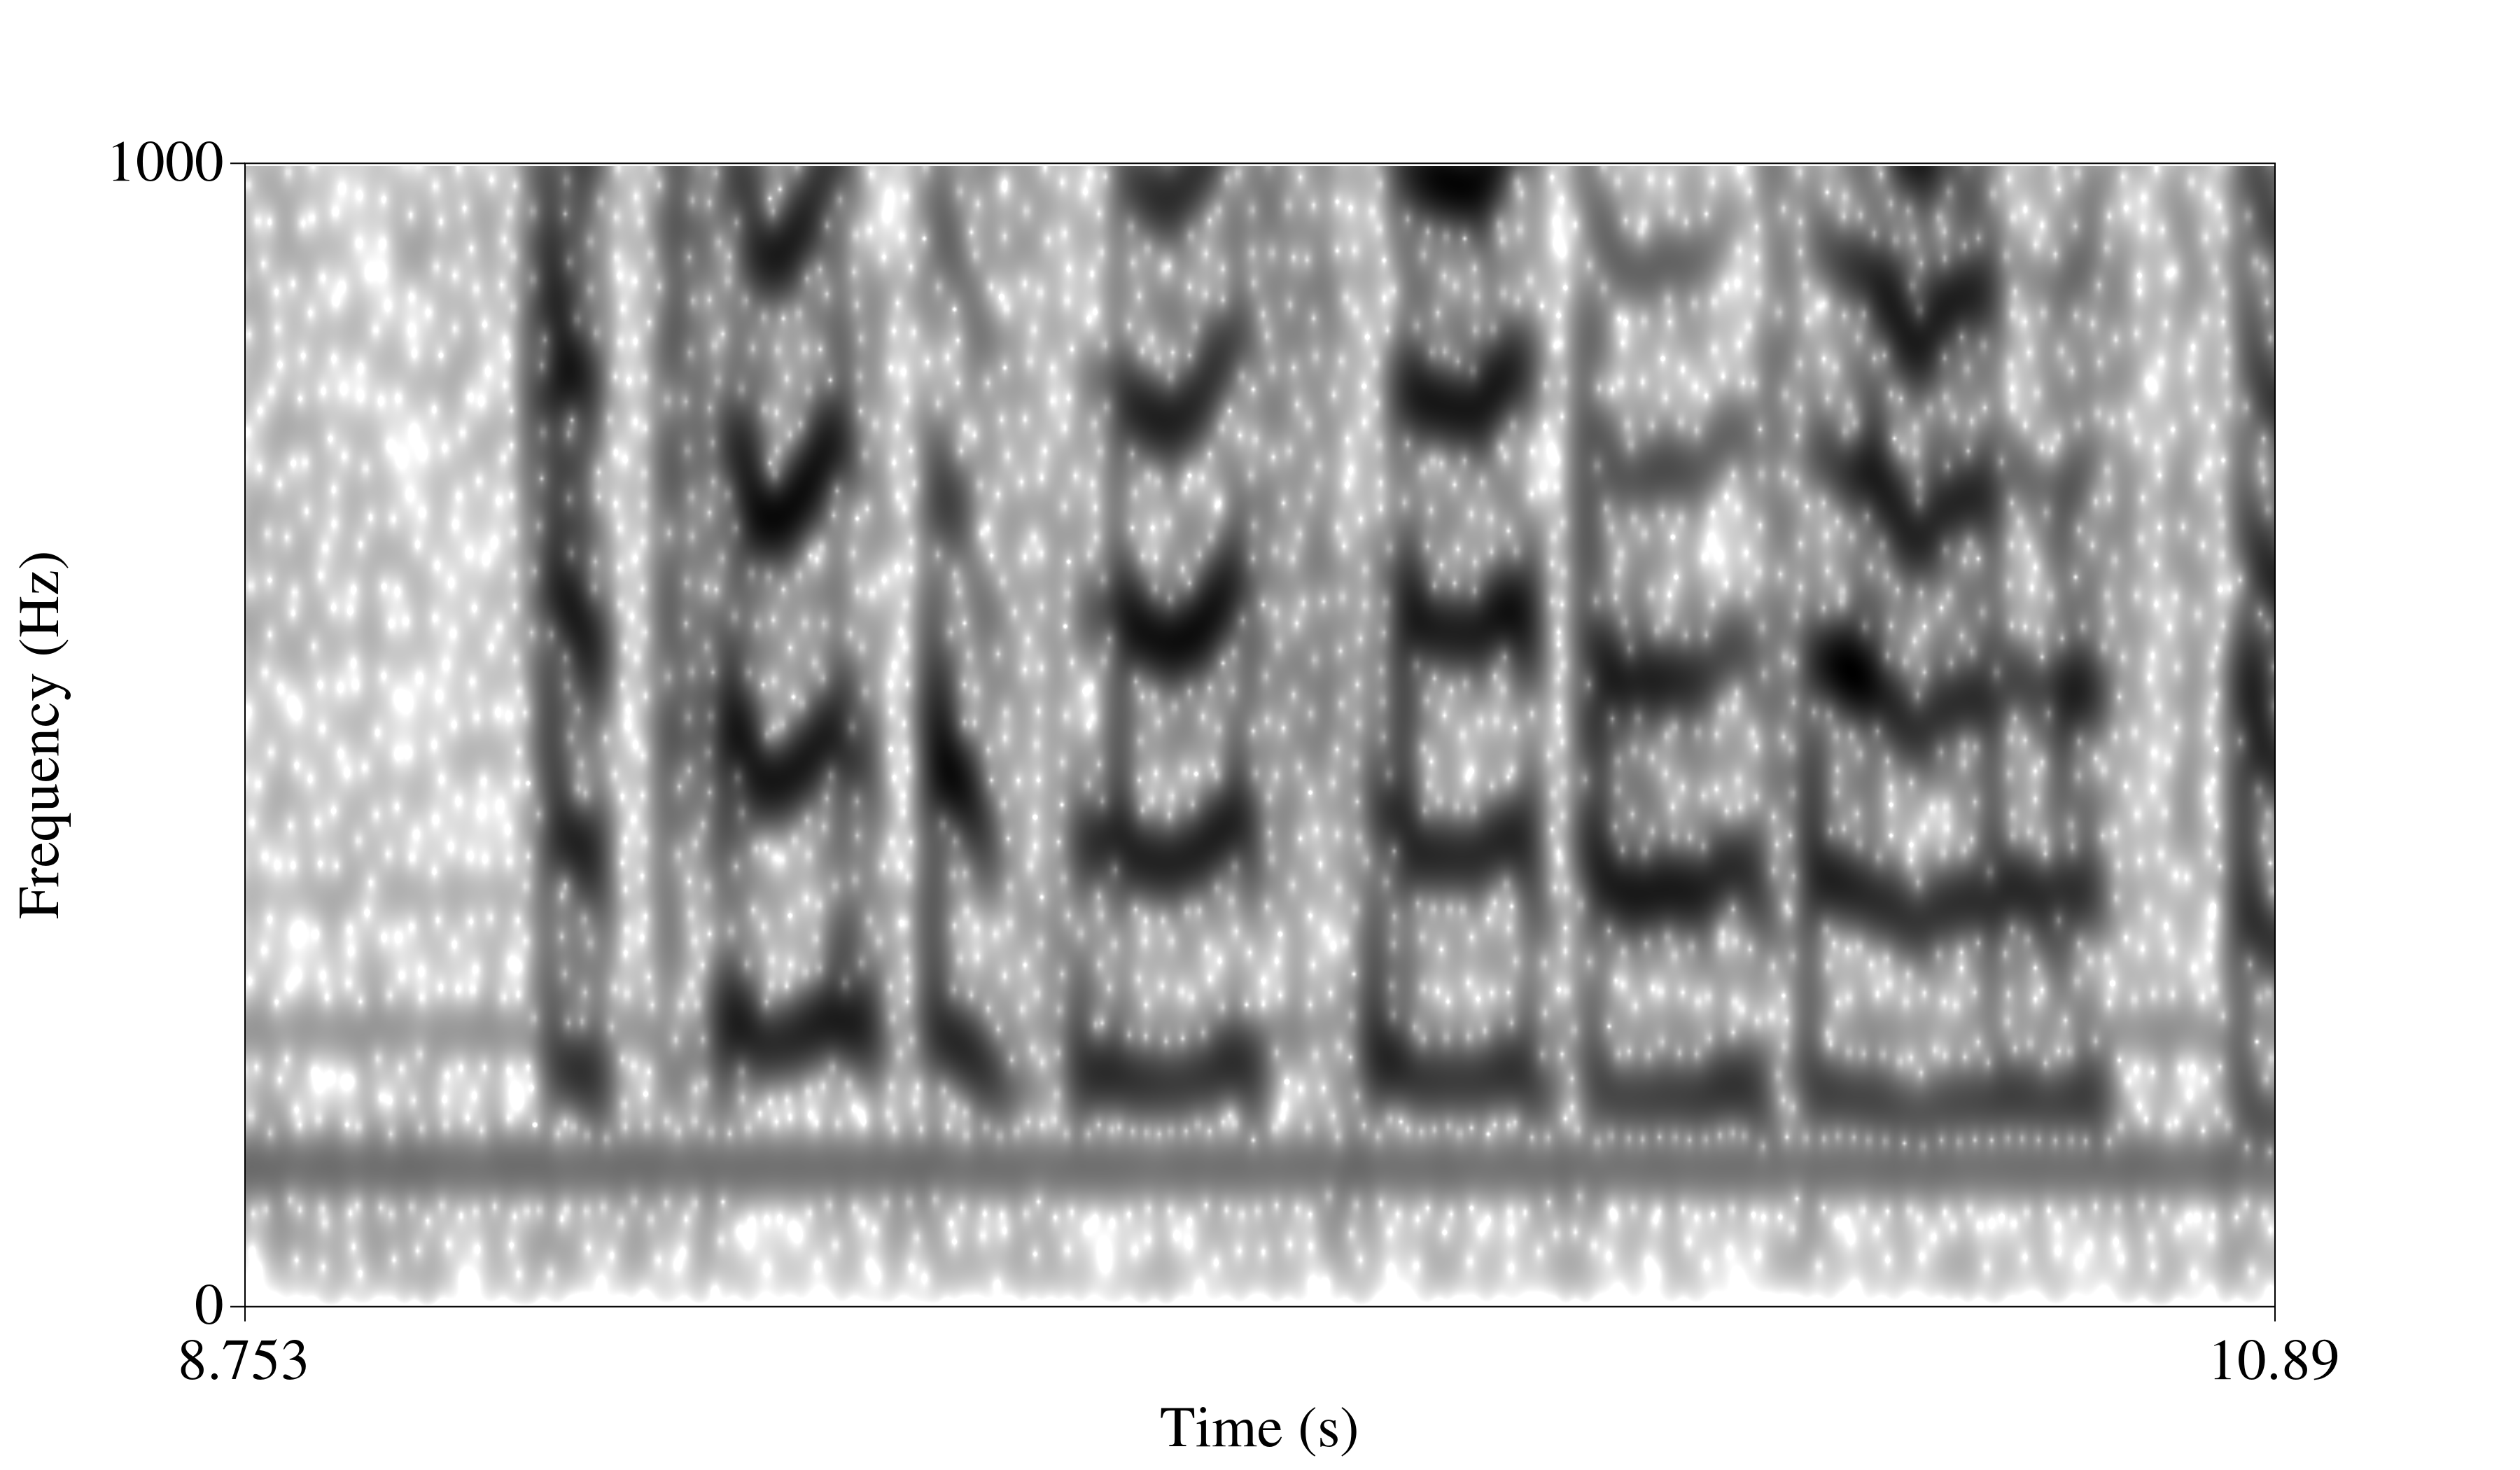
\includegraphics[width=1\linewidth]{figure/low_frequency_hum.png}
  \caption{The low frequency hum in the mouth-recorded signal.  It can be seen at 120 Hz and subsequent harmonics with decaying amplitude.}
  \label{fig:low_freq_hum-mouth}
\end{subfigure}%
\hfill
\begin{subfigure}{0.475\textwidth}
  \centering
  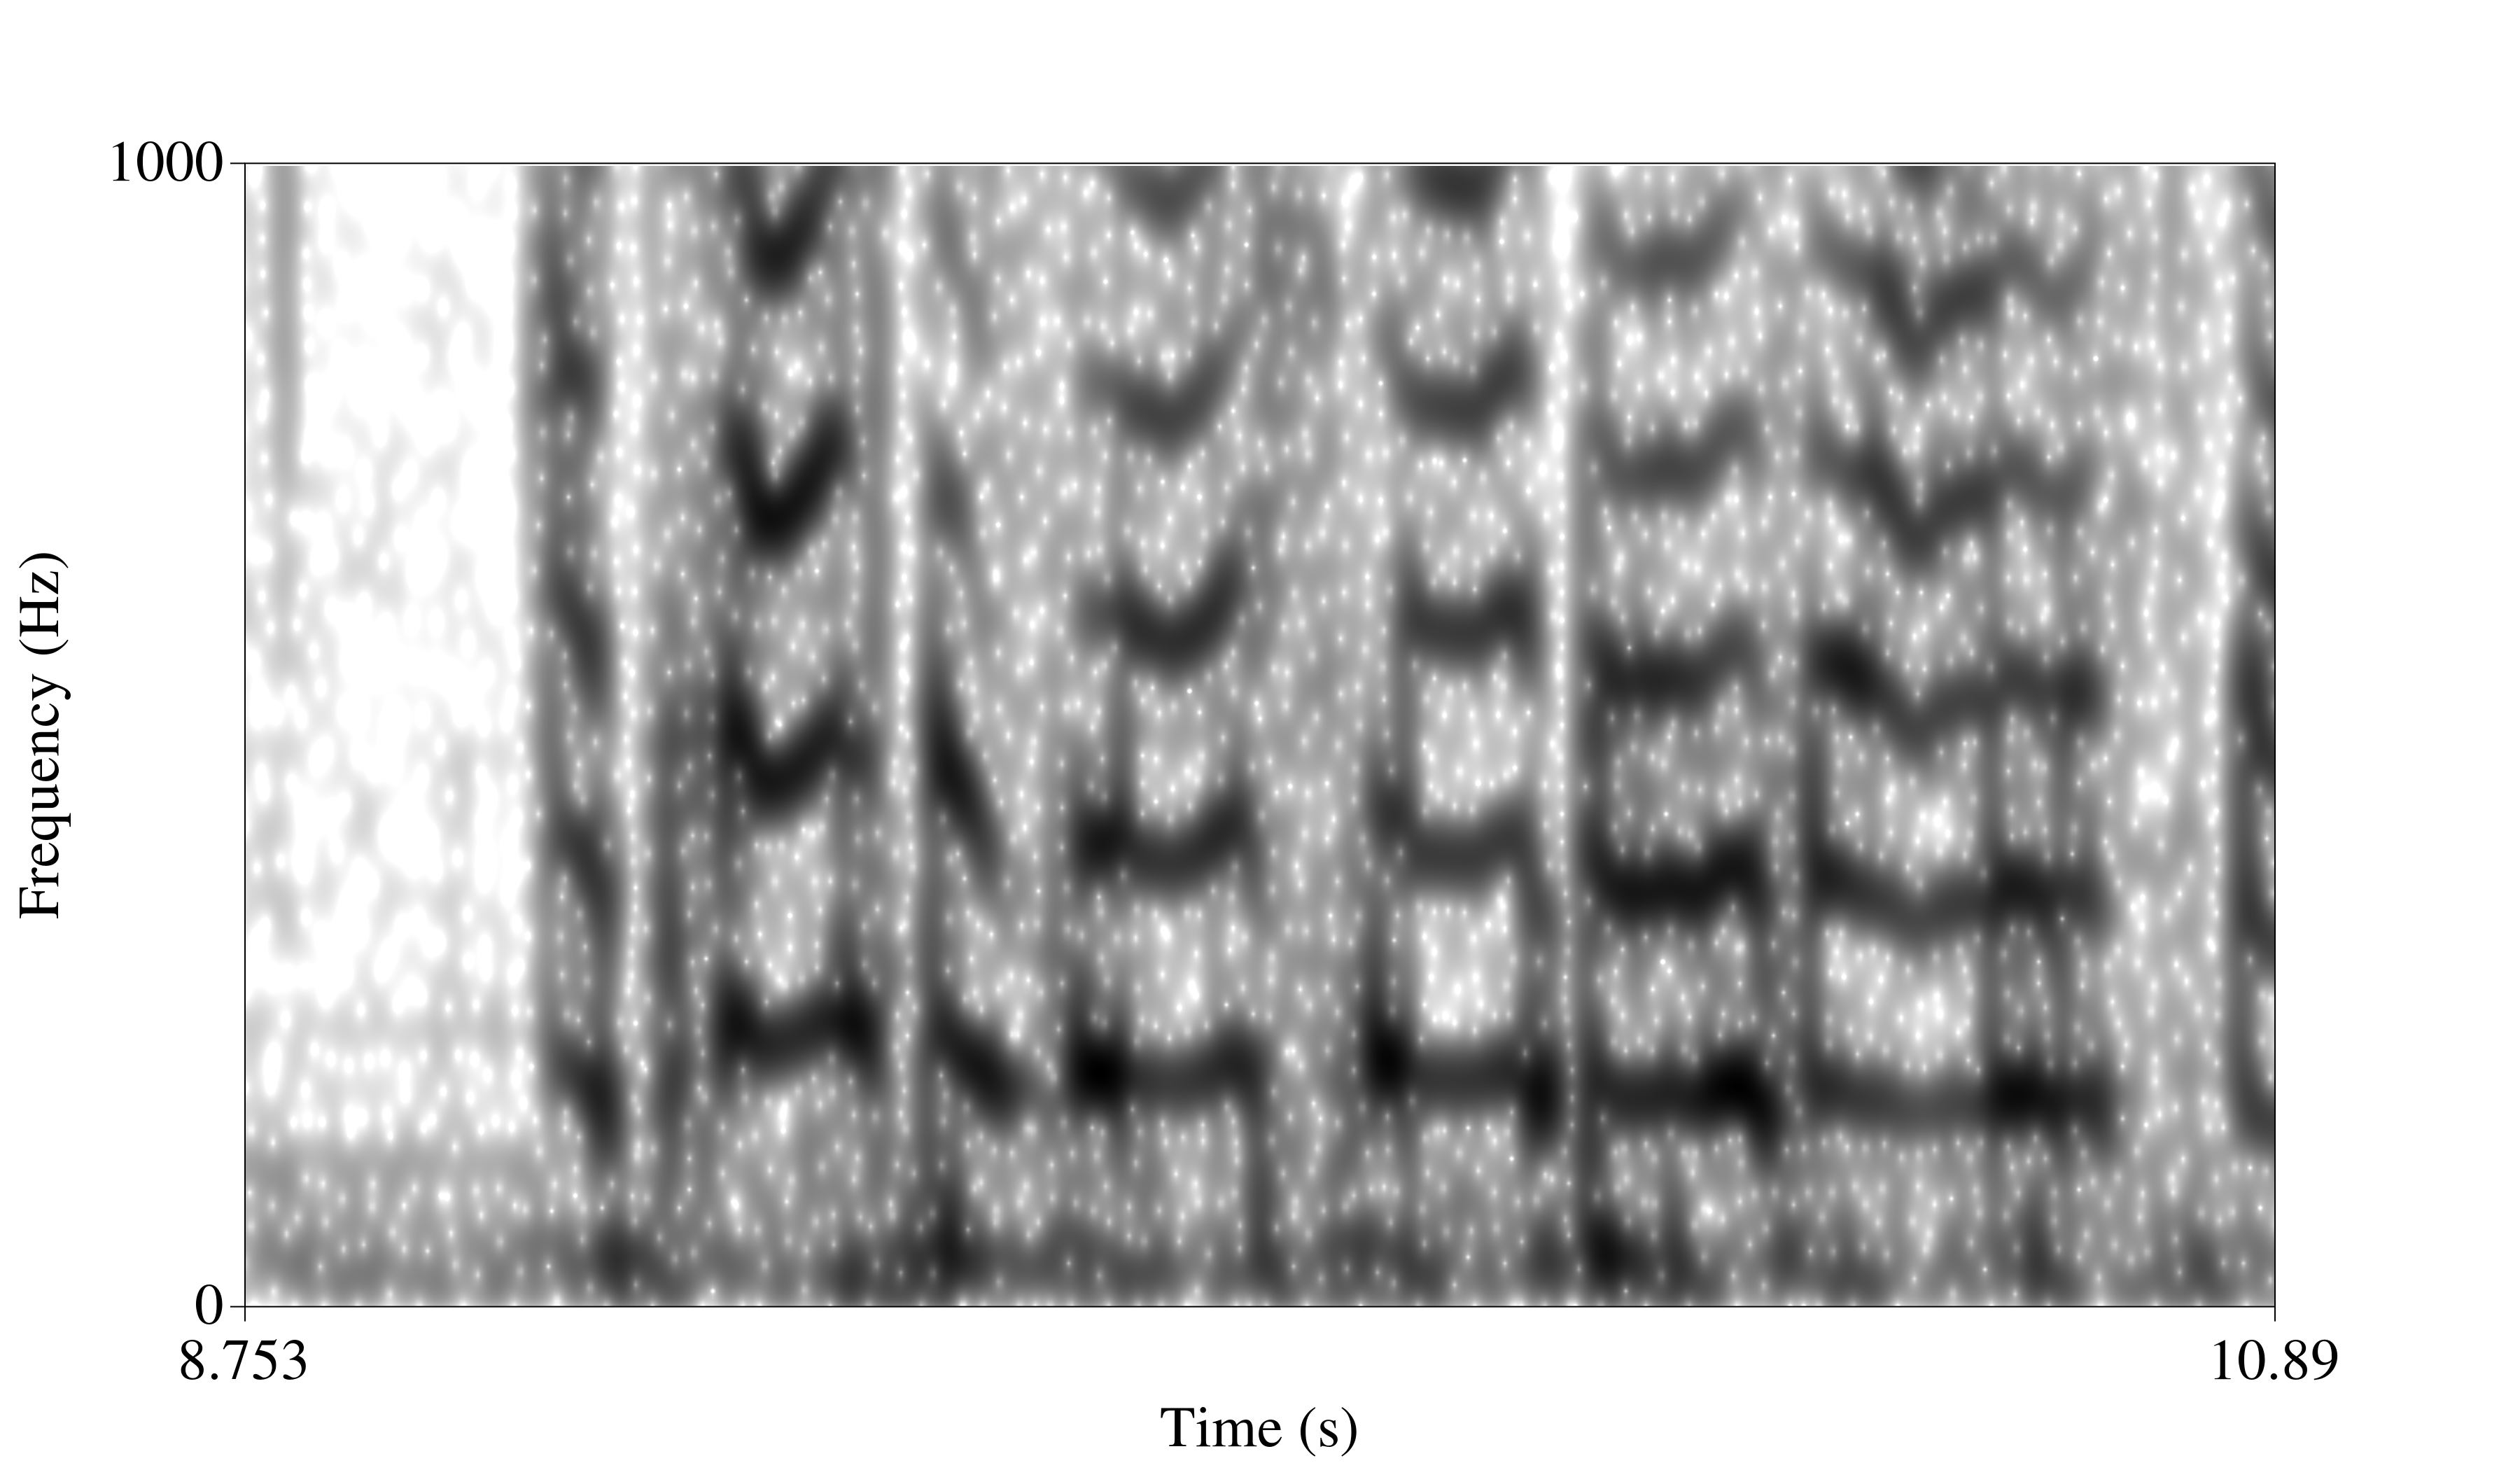
\includegraphics[width=1\linewidth]{figure/low_frequency_hum-ear.png}
  \caption{The low frequency hum in the ear-recorded signal. As in Figure \ref{fig:low_freq_hum-mouth}, it can be seen at 120 Hz and subsequent harmonics.  It is less prominent due to the gain on the recorder being lower.}
  \label{fig:low_freq_hum-ear}
\end{subfigure}
\caption{Spectrograms of a low frequency hum introduced by the recorder at 120 Hz and subsequent harmonics in both mouth (Fig. \ref{fig:low_freq_hum-mouth}) and ear (Fig. \ref{fig:low_freq_hum-ear}) recorded signals. The range of frequency is 0-1kHz.}
\label{fig:low_freq_hum}
\end{figure}

On a physical level, the earplugs which were used are fairly standard audiological silicone earplugs, which were the correct size to fit the microphones that were used.  It is unknown the degree of noise damping these plugs have, as they are not inherently designed for noise reduction.  It is very likely that a better NRR earplug could be found and used in conjunction with the 30dB NRR earmuffs to achieve a greater noise reduction at even higher noise levels.

Also, as mentioned earlier, the primary limitation is that the background noise was not loud enough to be able to fit into the SNR ratios desired (+10 dB SNR, 0 dB SNR, -10 dB SNR).  Instead, what was recorded was an average (across all speakers) 31, 23, and 12 dB SNR for the 60, 70, and 80 dB condition, respectively; The 60 dB noise condition reached as high as +40 dB SNR, and the lowest 80 dB noise condition SNR was +5 dB. The three noise levels can be seen in the spectrograms in Figure \ref{fig:noise_level_limitation} for the bus background noise.  Note that the noise level can barely be observed in the lowest noise condition in Fig. \ref{fig:limitation_bus_60}.

The two options to remedy this would be to a) ask the participants to speak more quietly, or b) increase the volume of the loudspeaker.  Option (a) is more appealing, as it continues to keep the ambient noise outside the range of amplitude which could possibly damage hearing.  However, it is difficult for a participant to consciously modify their loudness, and keep that consistent for the duration of the experiment; the need to repeat sentences spoken above a certain amplitude would drastically increase the length of time of the experiment.  On top of this, it would be difficult for the researcher monitoring the speech to determine whether or not the speech was an appropriate loudness, particularly with the additive background noise.  

\begin{figure}[h]
\centering
\begin{subfigure}{0.475\textwidth}
  \centering
  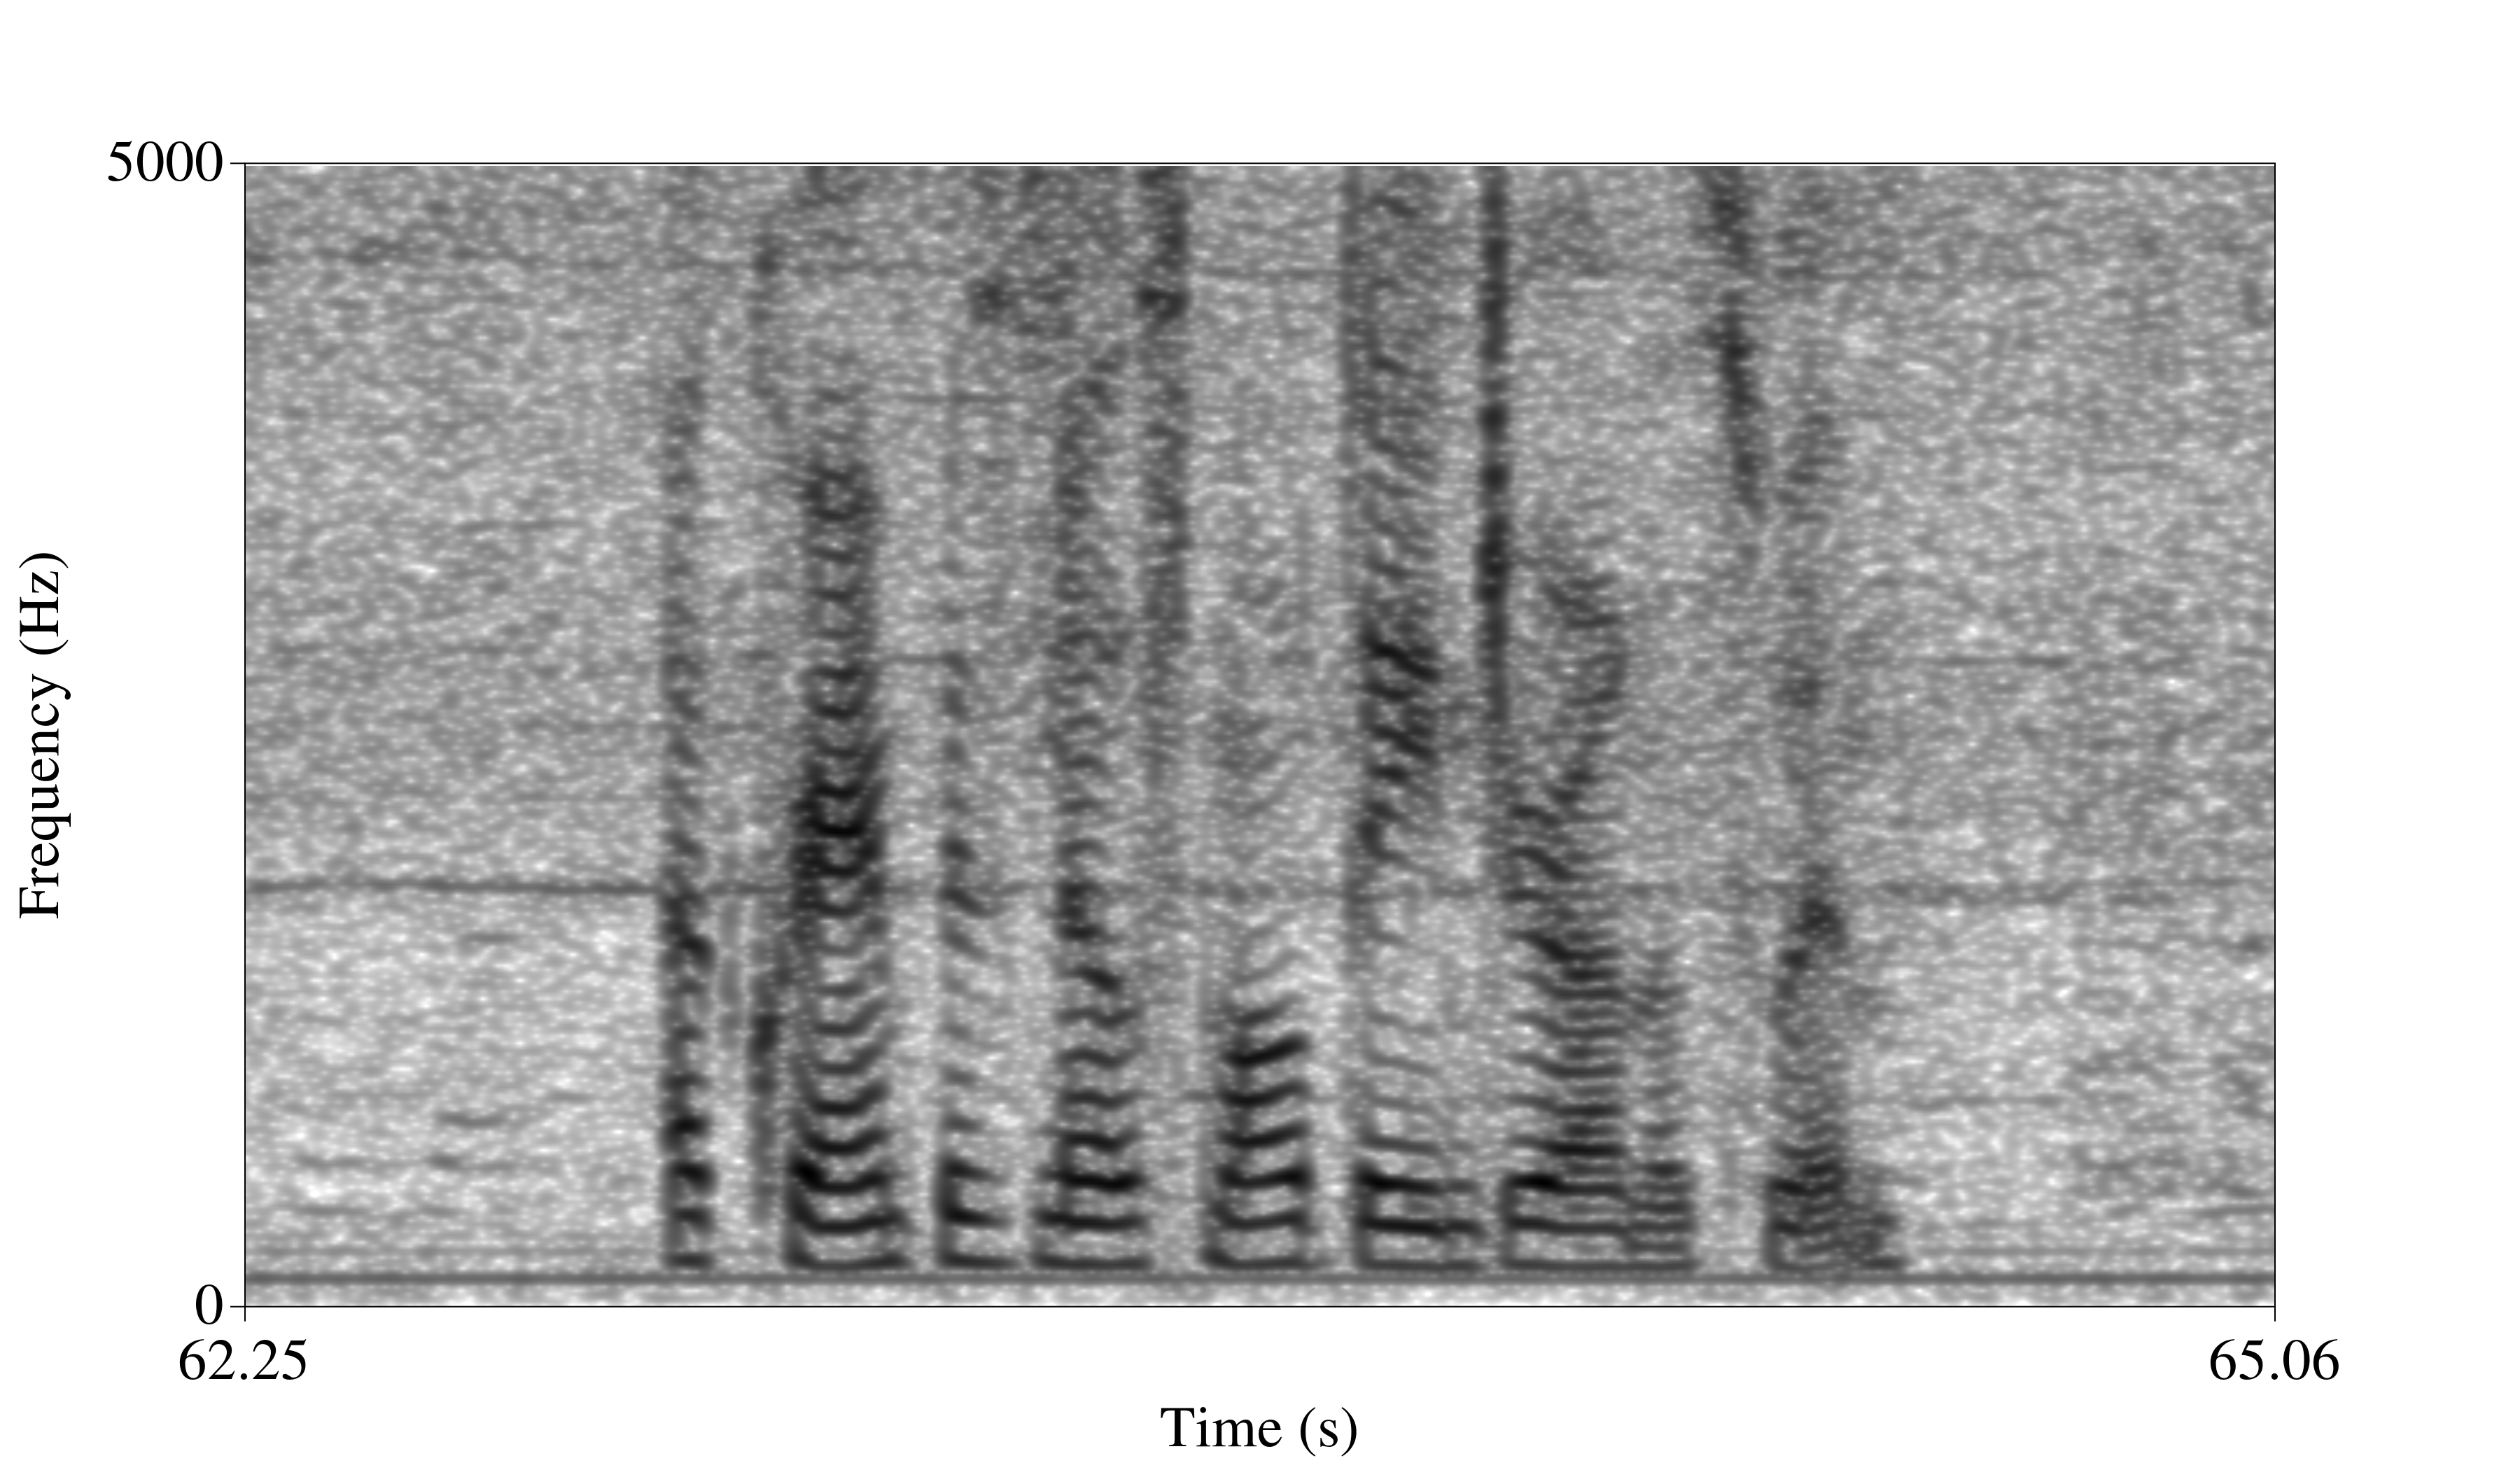
\includegraphics[width=1\linewidth]{figure/spctgrm_cramp_bus_60.png}
  \caption{The sentence ``A cramp is no small danger on a swim'' with bus background noise at 60 dB. SNR for this utterance is +28 dB.}
  \label{fig:limitation_bus_60}
\end{subfigure}%
\hfill
\begin{subfigure}{0.475\textwidth}
  \centering
  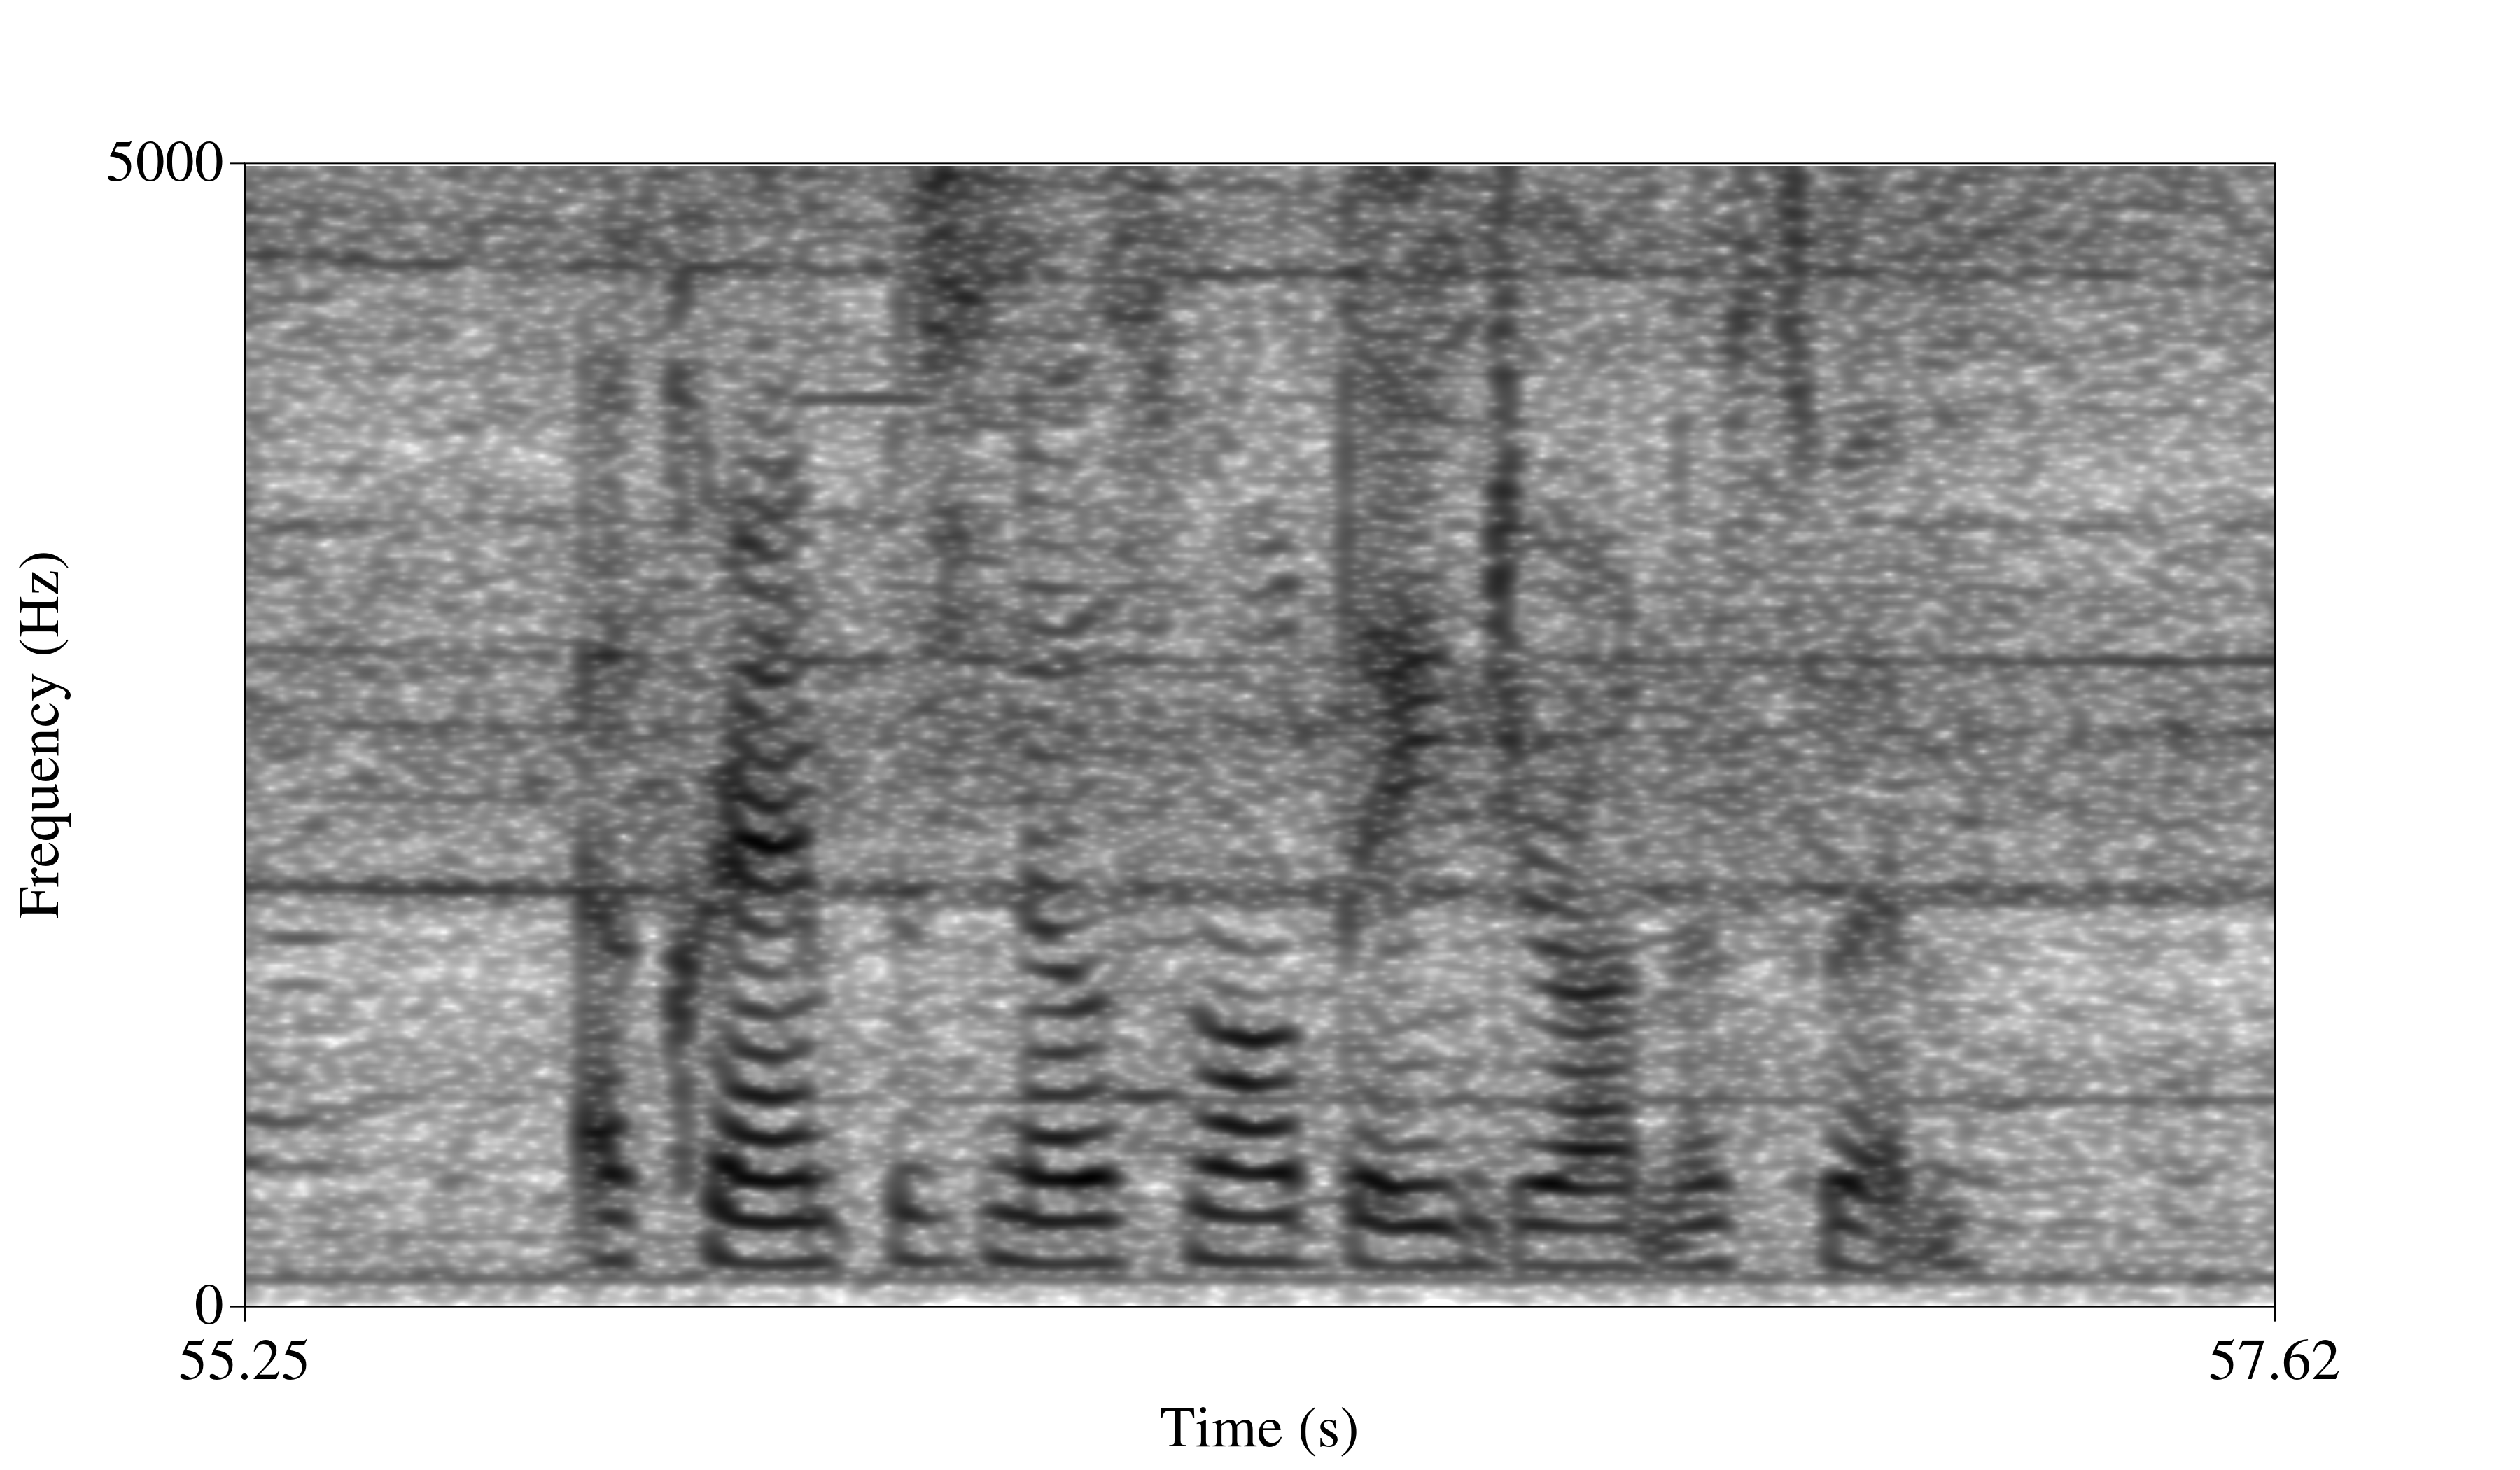
\includegraphics[width=1\linewidth]{figure/spctgrm_cramp_bus_70.png}
  \caption{The sentence ``A cramp is no small danger on a swim'' with bus background noise at 70 dB. SNR for this utterance is +19 dB.}
  \label{fig:limitation_bus_70}
\end{subfigure}
%
\begin{center}
\begin{subfigure}{0.475\textwidth}
  \centering
  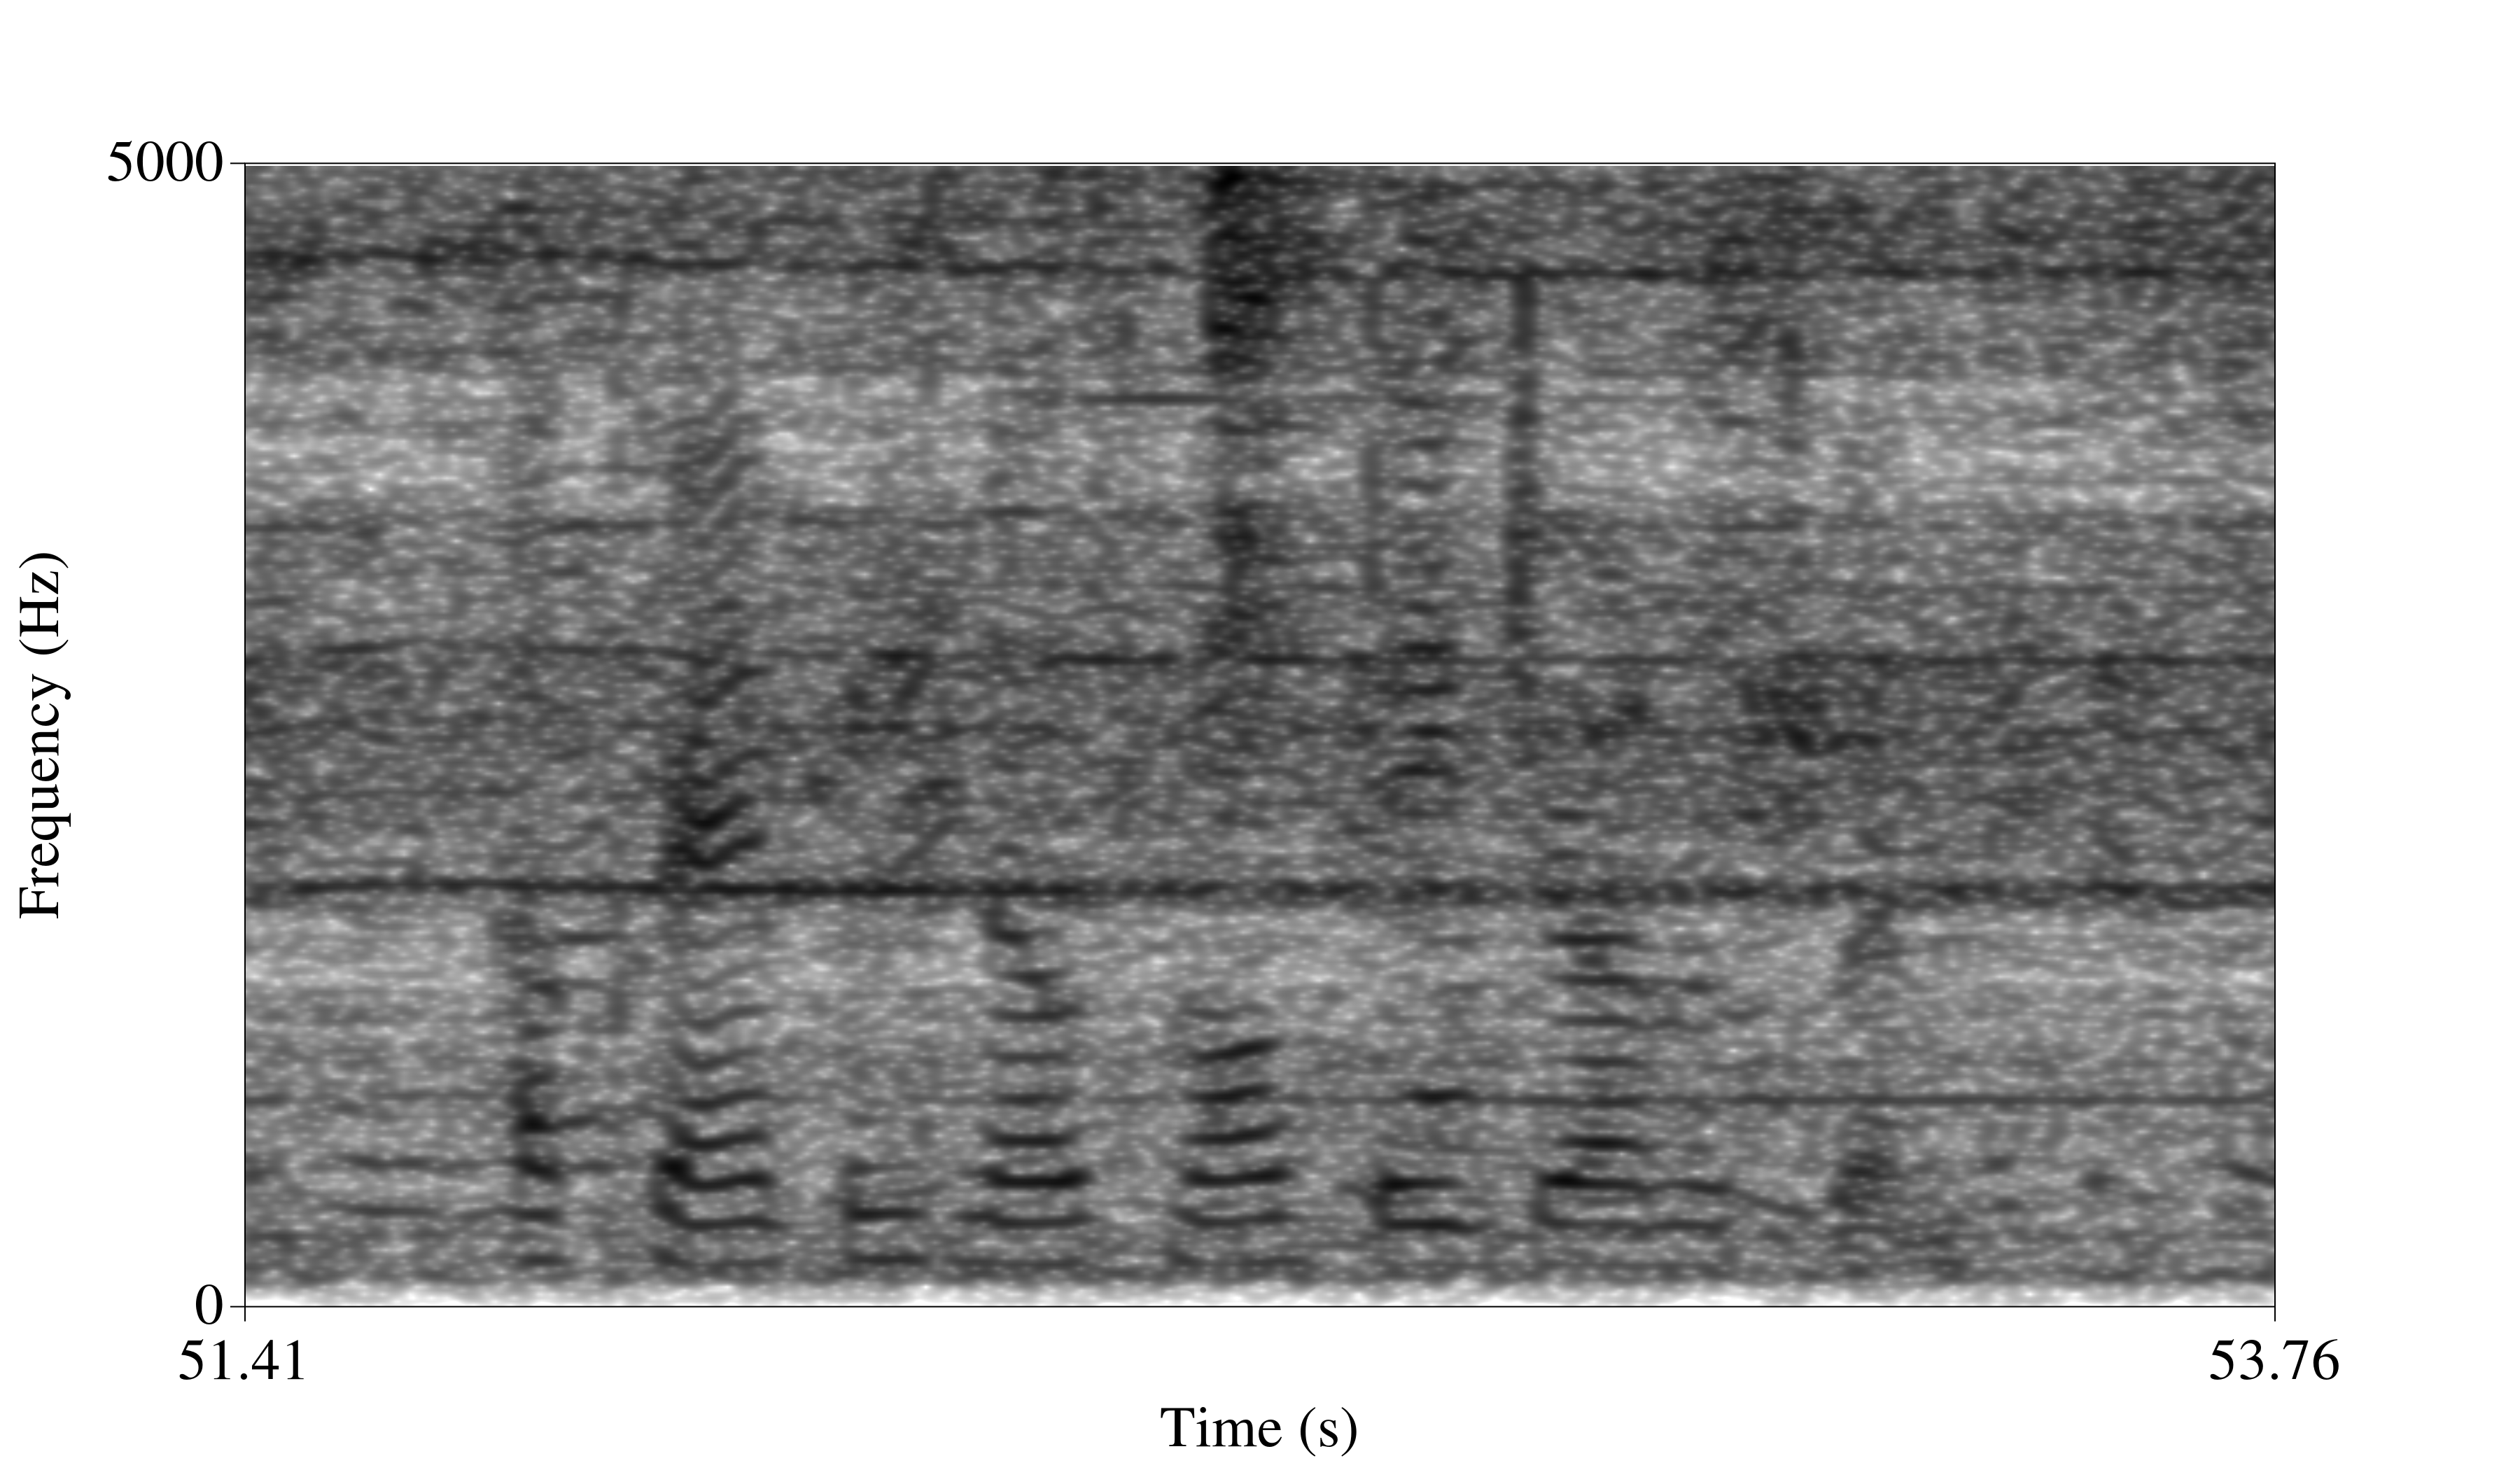
\includegraphics[width=1\linewidth]{figure/spctgrm_cramp_bus_80.png}
  \caption{The sentence ``A cramp is no small danger on a swim'' with bus background noise at 80 dB. SNR for this utterance is +6 dB.}
  \label{fig:limitation_bus_80}
\end{subfigure}
\end{center}
\caption{Spectrograms of the sentence ``A cramp is no small danger on a swim'' with bus background noise at 60 dB (\ref{fig:limitation_bus_60}), 70 dB(\ref{fig:limitation_bus_60}), and 80 dB (\ref{fig:limitation_bus_60}). The directional microphone filtered out most of the noise in the lower two noise level conditions.}
\label{fig:noise_level_limitation}
\end{figure}

Option (b) - increasing the noise level itself - is less appealing in that it results in a higher risk for hearing damage.  Given the SNR of +6dB for the 80dB noise condition (with some 80dB noise conditions having upwards of +10dB SNR), this would mean increasing the ambient noise from 80dB to 96-100dB in order to achieve the -10dB SNR that was originally desired.  Even a 0dB SNR would require a 90dB ambient noise to cover all speakers. The risk is mitigated by the use of 30dB NRR earmuffs, however at noises of this magnitude, it would be difficult to find a location which insulated the sound from affecting a significant radius outside the sound booth.  It is also very likely that a different loudspeaker would be required to reach that amplitude without clipping.

\subsection{Conclusions}

While there is some speaker variation, the speech recorded from inside the ear canal contains information up to approximately 2700Hz.  This upper cut-off frequency is in the same range described by the literature above.  Two, very basic acoustic transformations (pre-emphasis and bandpass filtering) were used in an attempt to create a more intelligible signal from the speech collected at the ear.
%, the heavily lowpass filtered speech becomes remarkably intelligible, considering the location of recording and the minimal post-processing effort required. 

%Given the relatively well-preserved lower frequency speech information that is present in the signal, no further acoustic transformation to these frequencies is deemed necessary\footnote{E.g. such as a spectral subtraction technique based on the frequency responses given in the literature by \cite{hansen:97b} and \cite{reinfeldt:10}, among others.}.  
Limited gains might be seen from a sound or sound-category specific alteration, particularly among fricative sounds and those with the majority of speech information located in frequencies above 2700Hz.  It seems unlikely though, that spectral subtraction (e.g. using the filters proposed by \cite{hansen:97b} and \cite{reinfeldt:10}) or a similar method would offer much additional benefit, as much of the upper frequencies were dampened beyond the existing noise level (c.f. fig \ref{spctgrmNarrowEarNoisePremp_35}).  However, it is hypothesized, given the transformed data collected at the ear, that enough information is present for the speech to be recognizable.  This hypothesis will be tested in a human perception experiment, described in Chapter \ref{chapter3}, and an ASR experiment, described in Chapter \ref{chapter4}, below.







\bibliographystyle{apa}
\bibliography{DissRefs.bib}
\end{document}
